% Version 0; preprint format; Outline of paper I by Song Huang

\documentclass[a4paper,fleqn,usenatbib]{mnras}

% Packages
\usepackage{url}
\usepackage{float}
\usepackage{natbib}
\usepackage{hhline}
\usepackage{multirow}
\usepackage{hyperref}
\usepackage{graphicx}
\usepackage{ae,aecompl}
\usepackage[T1]{fontenc}
\usepackage{deluxetable}
\usepackage{amssymb, amsmath}
\usepackage{newtxtext,newtxmath}
\usepackage[usenames, dvipsnames]{xcolor}
\usepackage{xcolor,colortbl}

% Package Settings
\hypersetup{colorlinks=true,
            citecolor=MidnightBlue,
            linkcolor=MidnightBlue,
            filecolor=magenta,
            urlcolor=cyan}
\urlstyle{same}

% Figure extention
\DeclareGraphicsExtensions{.pdf,.png,.jpg}

% User definitons
%--------------- User Defined Commands ---------------------%
% Past papers
\defcitealias{Huang2018b}{Paper~I}	
\defcitealias{Huang2018c}{Paper~II}	


% Journals
\def\aa{{A\&A}}
\def\aas{{ A\&AS}}
\def\aj{{AJ}}
\def\annrev{{ARA\&A}}
\def\apj{{ApJ}}
\def\apjs{{ApJS}}
\def\mnras{{MNRAS}}
\def\nat{{Nature}}
\def\pasp{{PASP}}

% Song Huang's definition 
\def\arcsec{{\prime\prime}}
\def\arcmin{{\prime}}
\def\degree{{\circ}}
\def\h{\hskip -3 mm}
\def\amin{$^\prime$}
\def\asec{$^{\prime\prime}$}
\def\deg{$^{\circ}$}
\def\ddeg{{\rlap.}$^{\circ}$}
\def\dsec{{\rlap.}$^{\prime\prime}$}
\def\cc{cm$^{-3}$}
\def\flamb{erg s$^{-1}$ cm$^{-2}$ \AA$^{-1}$}
\def\flux{erg s$^{-1}$ cm$^{-2}$}
\def\fnu{erg s$^{-1}$ cm$^{-2}$ Hz$^{-1}$}
\def\hst{{\textit{HST}}}
\def\kms{km s$^{-1}$}
\def\lamb{$\lambda$}
\def\lax{{$\mathrel{\hbox{\rlap{\hbox{\lower4pt\hbox{${\sim}$}}}\hbox{$<$}}}$}}
\def\gax{{$\mathrel{\hbox{\rlap{\hbox{\lower4pt\hbox{${\sim}$}}}\hbox{$>$}}}$}}
\def\simlt{\lower.5ex\hbox{$\; \buildrel < \over {\sim} \;$}}
\def\simgt{\lower.5ex\hbox{$\; \buildrel > \over {\sim} \;$}}
\def\micron{{$\mu$m}}
\def\perang{\AA$^{-1}$}
\def\peryr{yr$^{-1}$}
\def\lsun{$L_\odot$} 
\def\sigs{$\sigma_*$}
\def\etal{{\ et al.}}
\newcommand{\lt}{<}
\newcommand{\gt}{>}

% ---- Commonly used notations ---- %
\def\mlratio{{$M_{\star}/L_{\star}$}}
\def\snratio{{$\mathrm{S}/\mathrm{N}$}}
\def\mden{{$\mu_{\star}$}}
\def\sb{mag~arcsec$^{-2}$}
\def\ser{{S\'{e}rsic}}
\def\cmodel{\texttt{CModel}}
\def\cmod{\texttt{CModel}}

% ----- COMMON NOTATIONS ABOUT MASS ----- %
\def\msun{$M_\odot$}
\def\mstar{{$M_{\star}$}}
\def\logms{{$\log_{10} (M_{\star}/M_{\odot})$}}
\def\logmh{{$\log_{10} (M_{\mathrm{Vir}}/M_{\odot})$}}
\def\logmvir{{$\log_{10} M_{\mathrm{vir}}$}}
\def\logmpeak{{$\log_{10} M_{\mathrm{peak}}$}}
\def\logminn{{$\log_{10} (M_{\star,10\mathrm{kpc}}/M_{\odot})$}}
\def\logmtot{{$\log_{10} (M_{\star,100\mathrm{kpc}}/M_{\odot})$}}
\def\logmout{{$\log_{10} (M_{\star,150\mathrm{kpc}}/M_{\odot})$}}
\def\logmmax{{$\log_{10} (M_{\star,\mathrm{max}}/M_{\odot})$}}
\def\logmcen{{$\log_{10} (M_{\star,\mathrm{cen}}/M_{\odot})$}}
\def\logmcmodel{{$\log_{10} (M_{\star,\mathrm{CMod}}/M_{\odot})$}}
\def\logm10{{$\log (M_{\star,10\ \mathrm{kpc}}/M_{\odot})$}}
\def\logm30{{$\log (M_{\star,30\ \mathrm{kpc}}/M_{\odot})$}}
\def\logm50{{$\log (M_{\star,50\ \mathrm{kpc}}/M_{\odot})$}}
\def\logm100{{$\log (M_{\star,100\ \mathrm{kpc}}/M_{\odot})$}}
\def\logmtot{{$\log (M_{\star,\mathrm{tot}}/M_{\odot})$}}
\def\logmsim{{$\log (M_{\star,\mathrm{3D}}/M_{\odot})$}}

% Stellar mass of all galaxies in the halo
\def\mall{{$M_{\star,\mathrm{all}}$}}
\def\mcen{{$M_{\star,\mathrm{cen}}$}}
\def\mgal{{$M_{\star,\mathrm{gal}}$}}
\def\mins{{$M_{\star,\mathrm{ins}}$}}
\def\mexs{{$M_{\star,\mathrm{exs}}$}}

% ---- Key definitions of halo mass ---- %
\def\mvir{{$M_{\mathrm{vir}}$}}
\def\mhalo{{$M_{\mathrm{vir}}$}}
\def\mpeak{{$M_{\mathrm{peak}}$}}
\def\mhost{{$M_{\mathrm{200b}}$}}
\def\mh200b{{$M_{\mathrm{200b}}$}}
\def\mh200c{{$M_{\mathrm{200c}}$}}

% ---- Aperture Stellar Mass ---- %
\newcommand{\maper}[1]{\ensuremath{M_{\star, {#1}\ \rm kpc}}}
\newcommand{\logmaper}[1]{{$\log (M_{\star, {#1}\ \rm kpc}/M_{\odot})$}}

\newcommand{\menve}[2]{{$M_{\star, [#1, #2]}$}}
\newcommand{\logmenve}[2]{{$\log (M_{\star, [#1, #2]}/M_{\odot})$}}

% Use italic font for in situ and ex situ
\def\insitu{{\textit{in situ}}}
\def\exsitu{{\textit{ex situ}}}
\def\ins{{\textit{in situ}}}
\def\exs{{\textit{ex situ}}}

% ---- Related to scatters of SHMR ---- %
% Scatter of log-M*_all at fixed halo mass (using stellar mass of all galaxies)
\def\sigms{{$\sigma_{M_{\star}}$}}
% Scatter of log-M*_cen at fixed halo mass (using stellar mass of central galaxies)
\def\sigmcen{{$\sigma_{\log M_{\star, {\rm cen}}}$}}
% Scatter of log-Mpeak at fixed stellar mass
\def\sigmpeak{{$\sigma_{\log M_{\mathrm{peak}}}$}}
% Scatter of log-M200b at fixed stellar mass
\def\sigmh{{$\sigma_{M_{\mathrm{vir}}}$}}
%\def\sigmh{{$\sigma_{\mathcal{M} | \mathcal{O}}$}}
% Scatter of log-Mvir at fixed stellar mass
\def\sigmvir{{$\sigma_{M_{\mathrm{vir}}}$}}
%\def\sigmvir{{$\sigma_{\mathcal{M} | \mathcal{O}}$}}


% ---- Fractions used in the model ---- %
% Ratio between the stellar mass of a galaxy and the stellar mass
% of all galaxies in the same halo
\def\fgal{{$\delta_{\rm gal}$}}
\def\fcen{{$\delta_{\rm cen}$}}
% Fraction of the in-situ component in stellar mass
\def\fins{{$\delta_{\rm ins}$}}
% Fraction of the ex-situ component in stellar mass 
\def\fexs{{$\delta_{\rm exs}$}}

% ---- Observed stellar mass from HSC images ---- %
% The 10 kpc aperture mass
\def\minn{{$M_{\star,10\ \mathrm{kpc}}$}}
% The 100 kpc aperture mass
\def\mtot{{$M_{\star,100\ \mathrm{kpc}}$}}
% The maximum 1-D profile mass
\def\mmax{{$M_{\star,\mathrm{max}}$}}
% Stellar mass measured by CModel
\def\mcmodel{\ensuremath{M_{\star,\mathrm{cmod}}}}
% \def\mcmodel{\ensuremath{M_{\star,\mathrm{cmod}}}}
% ASAP predicted halo mass
\def\masap{{$M_{\rm vir,\ ASAP}$}}

% Project related or softwares
\def\um{\texttt{UniverseMachine}}
\def\htools{\texttt{halotools}}
\def\smdpl{\texttt{SMDPL}}
\def\mdpl2{\texttt{MDPL2}}
\def\rockstar{\texttt{Rockstar}}
\def\emcee{\texttt{emcee}}
\def\asap{\texttt{ASAP}}
\def\redm{\texttt{redMaPPer}}
\def\camira{\texttt{CAMIRA}}
\def\galfit{{\tt GALFIT}}
\def\ised{{\tt iSEDfit}}
\def\mblack{{\tt MassiveBlackII}}
\def\illustris{{\tt Illustris}}
\def\tng{{\tt Illustris--TNG}}
\def\ellipse{\texttt{Ellipse}}
\def\iraf{\texttt{IRAF}}
\def\hscpipe{\texttt{hscPipe}}
\def\topn{{Top-$N$}}

% ---- Weak lensing related ---- %
\def\dsigma{{$\Delta\Sigma$}}
\def\rdsigma{{$R \times \Delta\Sigma$}}
\def\chisq{{$\chi^2$}}
\def\sqdeg{{deg$^2$}}

% ----- Editing and commenting ----- %
% Color
\definecolor{LightGray}{gray}{0.85}
\definecolor{Tab1}{RGB}{114, 158, 206}
\definecolor{Tab2}{RGB}{255, 158,  74}
\definecolor{Tab3}{RGB}{103, 191,  92}
\definecolor{Tab4}{RGB}{174, 199, 232}
\definecolor{Tab5}{RGB}{255, 187, 120}
\definecolor{Tab6}{RGB}{152, 223, 138}
\definecolor{Tab7}{RGB}{255, 152, 150}
\definecolor{Tab8}{RGB}{197, 176, 213}
\definecolor{hpurple}{HTML}{7E16DF}

% CB commands
%\newcommand{\M}[1]{\ensuremath{M_{\ast,\,\rm #1}}} % \, is a little space
\newcommand{\scatterMstarx}[1]{\ensuremath{\sigma_{\M{#1} | \Mhalo{}}}}
\newcommand{\Mhalo}{\ensuremath{M_{\rm vir}}} 
\newcommand{\obsSym}{\ensuremath{{\mathcal{O}}}}
\newcommand{\haloSym}{\ensuremath{{\mathcal{M}}}}
\newcommand{\slope}{\ensuremath{\alpha}}
\newcommand{\intercept}{\ensuremath{\pi}}
\newcommand{\hmf}{\Phi(\mu)}
\newcommand{\scatterObsSymMhalo}{\ensuremath{\sigma_{\mathcal{O} | \mathcal{M}}}}
\newcommand{\scatterMhaloObsSym}{\ensuremath{\sigma_{\mathcal{M} | \mathcal{O}}}}
\newcommand{\eg}{{\it e.g.,\/}}
\def\sighalo{{$\sigma_{M_{\rm vir}}$}}

% Commenting:
\newcommand{\xxx}[1]{\textcolor{red}{\textbf{XXX}}}
\newcommand{\todo}[1]{\textcolor{BrickRed}{\textbf{~#1}}}
\newcommand{\plan}[1]{\textcolor{Sepia}{#1}}
\newcommand{\addref}{{\textcolor{red}{REF}}}
\newcommand{\note}[2]{\textcolor{blue}{\textbf{[Comment (#1): #2]}}}
\newcommand{\alexie}[1]{\textcolor{blue}{\textbf{[Alexie: #1]}}}
\newcommand{\chris}[1]{\textcolor{PineGreen}{\textbf{[Chris: #1]}}}
\newcommand{\song}[1]{\textcolor{Cyan}{\textbf{[Song: #1]}}}
\newcommand{\susan}[1]{\textcolor{Bittersweet}{\textbf{[Susan: #1]}}}
\newcommand{\update}[1]{\textcolor{PineGreen}{#1}}
\newcommand{\aph}[1]{\textcolor{hpurple}{[APH: #1]}}
\newcommand{\jul}[1]{\textcolor{teal}{[JUL: #1]}}


%% ---------------------------------------------------------------------------------------------- %%
%% Title and Affiliations 
%% ---------------------------------------------------------------------------------------------- %%
\title[TopN Test]{
	Central Galaxy Mass: A Simple Tracer of Halo Mass with Scatter Comparable to 
	Richness and Reduced Projection Effects}
				  
\author[S. Huang et al.]{
        Song Huang$^{1,2}$\thanks{E-mail: sh19@princeton.edu (SH)},
        Christopher Bradshaw$^{2}$,
        Alexie Leauthaud$^{2}$,
        Andrew Hearin$^{3}$,
        \newauthor
        Peter Behroozi$^{4}$,
        Joseph DeRose$^{2}$,
        Johannes Lange$^{2}$,
        Jenny Greene$^{1}$,
        Joshua Speagle$^{5}$\\
        $^{1}$Department of Astrophysical Sciences, Peyton Hall,
              Princeton University, Princeton, NJ 08540, USA \\
        $^{2}$Department of Astronomy and Astrophysics, University of California 
              Santa Cruz, 1156 High St., Santa Cruz, CA 95064, USA\\
        $^{3}$Argonne National Laboratory, Argonne, IL 60439, USA\\
        $^{4}$Department of Astronomy and Steward Observatory, University of Arizona, 
              Tucson, AZ 85721, USA\\     
        $^{5}$Department of Astronomy, Harvard University, 60 Garden St, MS 46, 
              Cambridge, MA 02138, USA
        } 
          
%% ---------------------------------------------------------------------------------------------- %%
\date{Accepted XXX. Received YYY; in original form ZZZ}        
\pubyear{2020}                                  
  

%% ---------------------------------------------------------------------------------------------- %%
%% Header and Version 
%% ---------------------------------------------------------------------------------------------- %%

\begin{document}

\label{firstpage}
\pagerange{\pageref{firstpage}--\pageref{lastpage}}

\maketitle

%% ---------------------------------------------------------------------------------------------- %%
%% Abstract and Keywords 
%% ---------------------------------------------------------------------------------------------- %%

\begin{abstract}
          
    \plan{Placeholder: Massive haloes are useful to cosmology. But they are not easy to select 
    	  without introducing projection and mis-centering effect.
    	  Here we use HSC deep images and unprecedented weak lensing capability to 
    	  test the possibility of selecting the most massive dark matter halos using 
    	  just the central galaxies.
    	  }
    
\end{abstract}

% TODO: Need updates!
\begin{keywords}
    galaxies: elliptical and lenticular, cD --
    galaxies: formation --
    galaxies: photometry -- 
    galaxies: structure -- 
    galaxies: haloes
\end{keywords}


%% ---------------------------------------------------------------------------------------------- %%
%% Main Text
%% ---------------------------------------------------------------------------------------------- %%

%% ---------------------------------------------------------------------------------------------- %%
%% Introduction 
%% ---------------------------------------------------------------------------------------------- %%

\section{Introduction}
    \label{sec:intro}
    
    \todo{Outline by Alexie: Need to be updated}

    \begin{itemize}
    	
        \item \plan{The number counts of clusters is a sensitive probe of the dark matter halo mass 
            function and the growth of structure (Albrecht, Weinberg). 
            For this reason, and with the advent of large optical surveys (SDSS, CFHTenS, HSC, DES), 
            much effort has been focussed on the development of optical cluster finders. 
            Methods that have enjoyed the most success have been based on the identification of 
            the red sequence of cluster members (\redm{}, \camira{}).}
    	
    	\item \plan{\redm{} is a method that xxxx (refs). \camira{} does this xxx (refs).}
    	
        \item \plan{However, as more data has been collected and the precision of our measurements 
            has grown, a number of difficulties with red sequence cluster finding have begin to emerge. 
            Joe can help to write this section. The issues of projection effects. 
            And also forward modeling is hard because hard to model quenched galaxies. 
            Cite projection effect papers and DES cluster cosmology paper in prep.}
 
        \item \plan{In this paper, we use high signal-to noise weak lensing from the HSC survey 
            to test a number of alternative and potentially more simple tracers of halo mass. 
            As the core of this paper is the "top N test" \citep[][]{Reyes2008} 
            (Read this paper, is there a different name)? 
            The premise of this test is as follows xxx..}
   
        \item \plan{One of the alternative tracers of halo mass that we test is central galaxy 
            stellar mass. Traditionally, it has always been assumed that central galaxy mass is 
            a less desirable tracer of halo mass than richness because it has a larger scatter with 
            respect to halo mass (numbers go here). However, some of this scatter has been due 
            to poor measurements of the luminosities of super massive galaxies. Refs}
  
        \item \plan{Using deep high quality imaging from the HSC survey, 
            Huang et al showed that careful extractions of galaxy luminosity lead to lower 
            scatter in the stellar-to-halo mass relation that previously estimated. 
            Furthermore, Huang et al showed that not only galaxy total mass, but also 
            the shape of the galaxy light profile, also contains information about halo mass. 
            Given these recent developments, it is timely to conduct a direct comparison of 
            the new potentially quite simple tracers of halo mass with more traditional 
            tracers such as richness.}
    	
    \end{itemize}

%% ---------------------------------------------------------------------------------------------- %%
%% Structure of the paper 
%% ---------------------------------------------------------------------------------------------- %%
    
    \todo{Placeholder: Need to be updated}

    This paper is organized as follows. 
    We briefly go through the sample selection and data reduction processes in 
    \S \ref{sec:data}.  
    Please refer to \citetalias{Huang2018b} for more technical details.
    \S \ref{sec:dsigma} describes the weak lensing methodology, and the 
    measurements of aperture \mstar{} and \mden{} profiles are mentioned in 
    \S \ref{sec:method}.
    In \S \ref{sec:model}, we introduce an empirical model to describe the relation
    between stellar mass distribution and dark matter halo properties at 
    high-\mstar{} end. 
    Main results from the best--fit model are presented in \S \ref{sec:result} and 
    discussed in \S \ref{sec:discussion}. 
    Our summary and conclusions are presented in \S \ref{sec:summary}.

%% ---------------------------------------------------------------------------------------------- %%
%% Important assumptions and definitions
%% ---------------------------------------------------------------------------------------------- %%
    
    For cosmology, we assume $H_0$ = 70~km~s$^{-1}$ Mpc$^{-1}$, 
    ${\Omega}_{\rm m}=0.3$, and ${\Omega}_{\rm \Lambda}=0.7$.
    Stellar mass (\mstar{}) is derived using a Chabrier initial mass function 
    (IMF; \citealt{Chabrier2003}). 
    And we use $M_{\rm vir}$ for dark matter halo mass (\mhalo{}) as 
    defined in \citealt{BryanNorman1998}.
    
%% ---------------------------------------------------------------------------------------------- %%
%% Section: Data and Sample Selection
%% ---------------------------------------------------------------------------------------------- %%
\section{Data}
    \label{sec:data}

%% ---------------------------------------------------------------------------------------------- %%
%% S16A dataset
%% ---------------------------------------------------------------------------------------------- %%

\subsection{Hyper Suprime-Cam Survey Subaru Strategic Program}
    \label{sec:hsc}      

	\todo{Placeholder: copy from Paper I}

	%% General information
	
	In this work, we use the \texttt{WIDE} layer of the internal data release 
	\texttt{S16A} of the HSC SSP, an ambitious imaging survey using the new prime focus 
	camera on the 8.2--m Subaru telescope. 
	These data are reduced by \texttt{hscPipe 4.0.2}, a specially tailored version of 
	the Large Synoptic Survey Telescope (LSST) pipeline (e.g.\ \citealt{Juric2015}; 
	\citealt{Axelrod2010})\footnote{\url{https://pipelines.lsst.io}}, 
	modified for HSC (\citealt{HSC-PIPE}).
	The coadd images are $\sim$3--4 mag deeper than SDSS (Sloan Digital Sky Survey; 
	e.g., \citealt{SDSS-DR7, SDSS-DR8, SDSS-DR12}), with pixel scale of 0\asec{}$.168$
	and mean $i$-band seeing has FWHM of 0\asec{}$.58$.
	Please refer to \citet{HSC-SSP, HSC-DR1} for more details about the survey design
	and the data products.
	The general performance of \texttt{hscPipe} can be found in \citet{SynPipe}.
	In addition to the full--color and full--depth constrain, the effective survey 
	area also takes into account masks for bright stars described in
	\citet{HSC-STAR}.

%% ---------------------------------------------------------------------------------------------- %%
%% Massive Galaxy Sample
%% ---------------------------------------------------------------------------------------------- %%

\subsection{S16A Massive Galaxy Sample}
    \label{sec:sample}	

	\begin{itemize}
	
		\item From \texttt{S16A} dataset, we select a large sample of massive galaxies
			within the redshift range of $0.2 < z < 0.5$ and estimate their surface 
			stellar mass density profiles out to $>100$ kpc individually.
			This redshift range ensures the inner structure of a massive galaxy can be 
			well resolved while its outer stellar halo is still visible above the $i$-band
			surface brightness limit. 
			The cosmic volume it contains also ensures a statistically significant sample 
			of the most massive galaxies in nearby universe.
			Using the high-quality data from this sample, we revealed a remarkable structural
			diversity in the stellar halo of these massive galaxies and its connection to 
			the underlying \mhalo{} (\addref{}).
			Please see aforementioned papers for details about the data analysis processes.
			Here we will provide a summary of the sample selection and data analysis 
			process, please see aforementioned papers for more details.
			
		\item \plan{Initial selection}: We first select all HSC galaxies with CModel magnitude 
			brighter than $i_{\rm CMod} \leq 21.5$ mag. Based on previous analysis of massive 
			galaxies at similar redshift range, this generous flux cut ensures all massive
			galaxies with \mstar{}$>11.5$ are included (\addref{}).
			We then collect available spectroscopic redshift for this sample from a complied 
			list of spec-$z$ catalogs matched to HSC survey. 
			Most spec-$z$ are from SDSS/BOSS and GAMA surveys.
			We also cross-match the sample with the SDSS \redm{} and HSC S16A \camira{} 
			galaxy cluster catalogs. 
			These catalogs are based on the red-sequence method and can provide very accurate
			photometric redshift estimates for the central galaxy and other members of the
			clusters.
			For the rest galaxies, we adopt photometric redshifts based on the five-band
			HSC CModel photometry and the \texttt{FrankenZ} algorithm. \todo{Very brief mention
			of what is frankenz, and the precision}. Using photo-$z$ for the entire sample 
			does not change key results.
		
		\item \plan{SED fitting}: Based on the best-available redshift and CModel photometry, 
			we perform SED fitting using the IDL code \ised{}. 
			\plan{A little more details}.
			We compare the \mcmodel{} stellar mass function with the ones from similar 
			photometry including the CS82 and PRIMUS surveys. 
			We find good consistency at the high-mass end and confirm that the HSC 
			sample is complete at \mcmodel{}$>11.4$.
					
	\end{itemize}

%% ---------------------------------------------------------------------------------------------- %%
%% 1-D Surface Mass Density Profiles
%% ---------------------------------------------------------------------------------------------- %%

\subsection{1-D Surface Mass Density Profiles}
    \label{sec:1d_prof}

	\begin{itemize}
	
		\item Although the \cmod{} photometry provides a baseline stellar mass measurement,
			it is not an ideal stellar mass measurement to explore galaxy--halo connection.
			\plan{briefly mention the problem with CModel}.
			
		\item Therefore we perform our own 1-D surface brightness analysis to provide
			more accurate stellar mass estimates and to map the stellar mass 
			distribution in massive galaxies. 
			Using the \ellipse{} isophotal analysis function from \iraf{}, we carefully 
			extract 1-D $i$-band surface brightness profiles along the major axis of the 
			mean isophote of the galaxy. 
			Before the extraction, we aggressively mask out all neighboring objects, 
			empirically correct the local background when over-subtraction occurs, and 
			also test the method against a series of systematics. 
			On average, the 1-D surface brightness profile is robust from 5-6 kpc to 100 kpc.
			The central region suffers from smearing effect from seeing. 
			And the outer part often has $i$-band surface brightness level lower than 
			$\sim 28$ \sb{}, becoming much more vulnerable to background subtraction 
			and residual contaminations from nearby objects.
		
		\item Using the $i$-band \mlratio{} derived from SED fitting, we convert the 
			1-D surface brightness profile into surface stellar mass density profile.
            Through integrating these 1-D profiles within different radial ranges, we 
            can robustly estimate the \mstar{} stored within different apertures or 
            different parts of the galaxy.
            We should mention that all these \mstar{} are measured within elliptical 
            apertures that follow the shpe of the flux-weighted isophotal of the galaxy.
            Massive galaxies do have intrinsic \mlratio{} gradient, hence the assumption of 
            a constant \mlratio{} tends to slightly bias the \mstar{} measurements within 
            different radial ranges.
            In \citealt{Huang2018b}, we show that massive galaxies in our sample show
            color gradients that can be roughly translated into a shallow but negative 
            \mlratio{} gradient. 
            We also do not see evidence that suggests a \mstar{} or environment-depedence 
            of the color gradients.
            Although the \mlratio{} will not change any key result, it suggests that we
            could slightly under-estimate the stellar mass in the central region while
            over-estimating the \mstar{} in the outskirt when using the average \mlratio{}
            of the galaxy.

	\end{itemize}

%% ---------------------------------------------------------------------------------------------- %%
%% Key Methods used in this work
%% ---------------------------------------------------------------------------------------------- %%

\section{Methodology}
    \label{sec:method}
    
    In this section, we will outline the methodology adopted in this work to evaluate different 
    possible \mvir{} ``proxies'' using high-fidelity galaxy-galaxy lensing data and via
    comparison with empirical model of \mvir{}-observable scaling relation based on cosmological 
    N-body simulation.
    We will first introduce a series of \mstar{}- (\ref{sec:proxy_mstar}) and richness-based 
    (\ref{sec:proxy_richness}) \mvir{} tracers.
    Then we describe the measurement of the galaxy-galaxy lensing \dsigma{} (or excess surface 
    density, ESD) profiles using HSC \texttt{S16A} shape catalog (\ref{sec:dsigma}).
    In section \ref{sec:topn_intro}, we explain the philosophy of the ``Top N'' tests and the 
    choices of volume number density bins.

%% ---------------------------------------------------------------------------------------------- %%
%% Halo mass proxies based on stellar mass
%% ---------------------------------------------------------------------------------------------- %%

\subsection{\mstar{}-based Halo Mass Proxies}
    \label{sec:proxy_mstar}
    
    The stellar mass of the a galaxy has a well established physical relation with its halo mass.
    And more massive galaxies tend to live in more massive dark matter halos.
    Therefore it is natural to use \mstar{} of a galaxy as a first-order proxy of \mvir{}.
    In fact, the calibration of SHMR remains one of the focues in the study of galaxy-halo connection.
    However, the slope and scatter of SHMR at the high-\mstar{} still show discrepencies among 
    different constraints (\addref{}). 
    And the \mstar{} of a single galaxy is often considered a less accurate \mvir{} tracer 
    than many others, including the number of sub-halos (optical richness, \addref{}), 
    total luminosity or stellar mass within the halo (\addref{}), velocity dispersion of galaxies
    in the halo (\addref{}), and X-ray luminosity of a group or cluster (\addref{}). 
    
    But, we want to point out that 
    1) `\mstar{} measurement of one galaxy is a more straightforward approach and has seveal 
    appealing features. Observationly, it is more ``cost effective''. And it also suffers less
    from systematic issues such as the projection effect (\addref{}).
    2) In recent years, increasingly deep imaging surveys make us aware of the importance of the 
    faint stellar outskirt of massive galaxies (\addref{}). 
    After accounting for the \mstar{} in these diffuse stellar component closely tied to the 
    halo assembly, we could further improve the capability of using \mstar{} as a halo mass proxy.
    
    Here we introduce a list of \mstar{} options that will be explored in this work.

%% ---------------------------------------------------------------------------------------------- %%
%% CModel Stellar Mass
%% ---------------------------------------------------------------------------------------------- %%

\subsubsection{\cmodel{} stellar mass}
	\label{sec:mcmodel}

\subsubsection{Aperture \mstar{} from 1-D profile}
	\label{sec:maper}

\subsubsection{Outer envelope \mstar{}}
	\label{sec:menvelope}

\subsubsection{\mvir{} from \asap{} model}
	\label{sec:masap}

%% ---------------------------------------------------------------------------------------------- %%
%% Halo mass proxies based on optical richness
%% ---------------------------------------------------------------------------------------------- %%
\subsection{Richness-based proxies for Halo Mass}
	\label{sec:proxy_richness}


\subsubsection{\redm{} richness}
	\label{sec:redmapper}

\subsubsection{\camira{} richness}
	\label{sec:camira}

%% ---------------------------------------------------------------------------------------------- %%
%% Weak lensing measurements
%% ---------------------------------------------------------------------------------------------- %%
\subsection{\dsigma{} Profiles}
    \label{sec:dsigma}   
    
    \todo{Placeholder}
    
    	\begin{itemize}
		
		\item \plan{Copy something from the \asap{} paper.}
		
		\item \plan{Copy something from Speagle et al. 2019 here.}
		
	\end{itemize}    
       
%% ---------------------------------------------------------------------------------------------- %%
%% Introducing the TopN test and define the number density
%% ---------------------------------------------------------------------------------------------- %%
\subsection{``Top N'' Test and Number Density Bins}
    \label{sec:topn_intro}   

\todo{Placeholder}

%% ---------------------------------------------------------------------------------------------- %%
%% Section: Simulation and Model
%% ---------------------------------------------------------------------------------------------- %%
\section{Theoretical Models}
    \label{sec:model}

\subsection{Multi Dark Planck Simulation}

%% ---------------------------------------------------------------------------------------------- %%
%% Figure: Theoretical exploration of the relations among scatters and its impact on 
%%		   Delta Sigma profiles.
%% ---------------------------------------------------------------------------------------------- %%
\begin{figure*}
  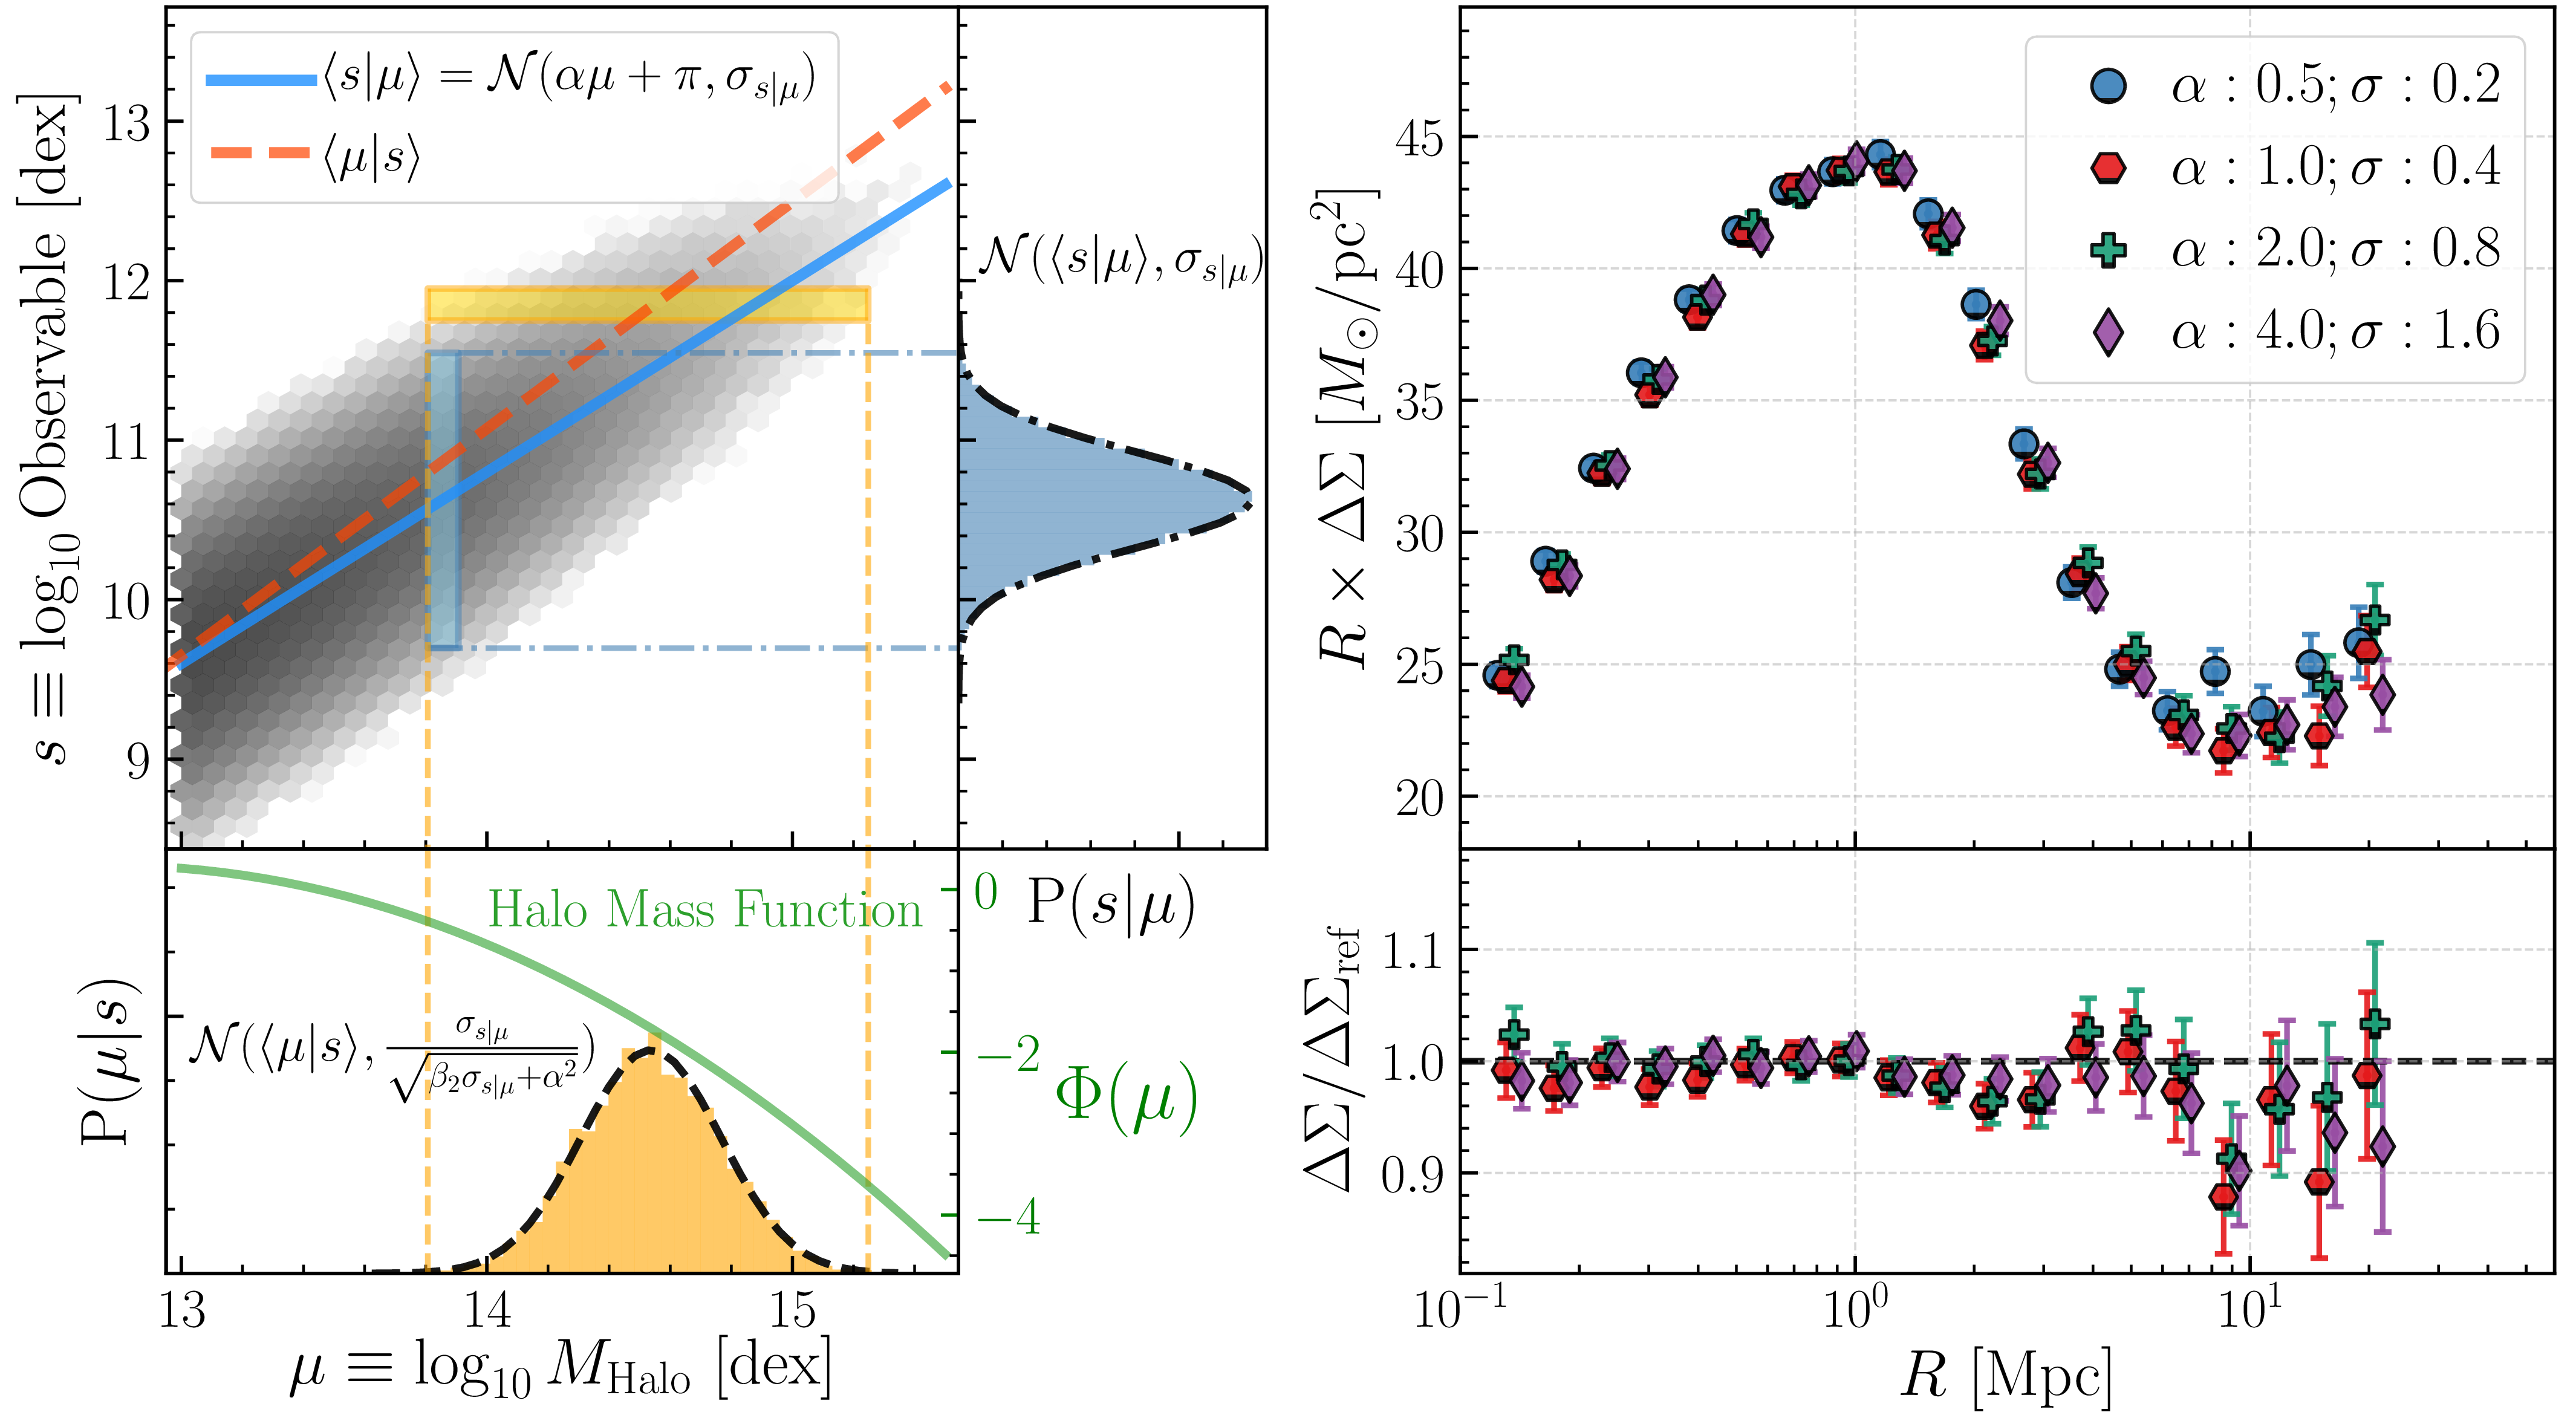
\includegraphics[width=\textwidth]{figure/theory.png}
  \caption{
     \textbf{Left}: The distribution of some observable, \obsSym{}, that is related to $\mu =
     \log(\Mhalo)$ by a linear relation with some scatter. By construction, $P(\obsSym | \mu)$
     (right panel, orange histogram) is normally distribution around $\langle \obsSym | \mu
     \rangle = \alpha \mu + \pi$ with a scatter of $\sigma_{\obsSym | \mu}$. The halo mass
     function (bottom panel, red line, right axis), is constructed using the best fit of a
     logarithmic quadratic (as in \ref{eq:quadratic_hmf}) to MDPL2. $P(\mu | \obsSym)$ (bottom
     panel, cyan histogram) is the distribution of $\mu$ given by a thin selection of \obsSym{}
     (main panel, cyan selection). This distribution of $\mu$ is well described by a normal
     distribution (green PDF) centered at the value given by \ref{eq:mean_of_mu} (cyan dashed
     line) with a scatter given by \ref{eq:scatter_of_mu} that depends on $\sigma_{\obsSym |
     \mu}$, the slope of the \obsSym - $\mu$ relation, $\alpha$, and the curvature of the mass
     function, $\beta_2$. The gap between $\langle \obsSym | \mu \rangle$ and $\langle \mu |
     \obsSym \rangle$ is smallest where the mass function is nearly flat (towards lower masses)
     while it becomes large at high masses where the steeper mass function leads to a large
     Eddington bias. \textbf{Right}: Observables with the same ratio $\alpha /
     \scatterObsSymMhalo$ have the same \scatterMhaloObsSym{} (see
     \ref{eq:ratio_is_what_matters}) and therefore the same DS profile.
	}
    \label{fig:theory}
\end{figure*}
%% ---------------------------------------------------------------------------------------------- %%

%% ---------------------------------------------------------------------------------------------- %%
%% Figure: Demonstration of the mock catalog
%% ---------------------------------------------------------------------------------------------- %%
\begin{figure*}
  \centering
  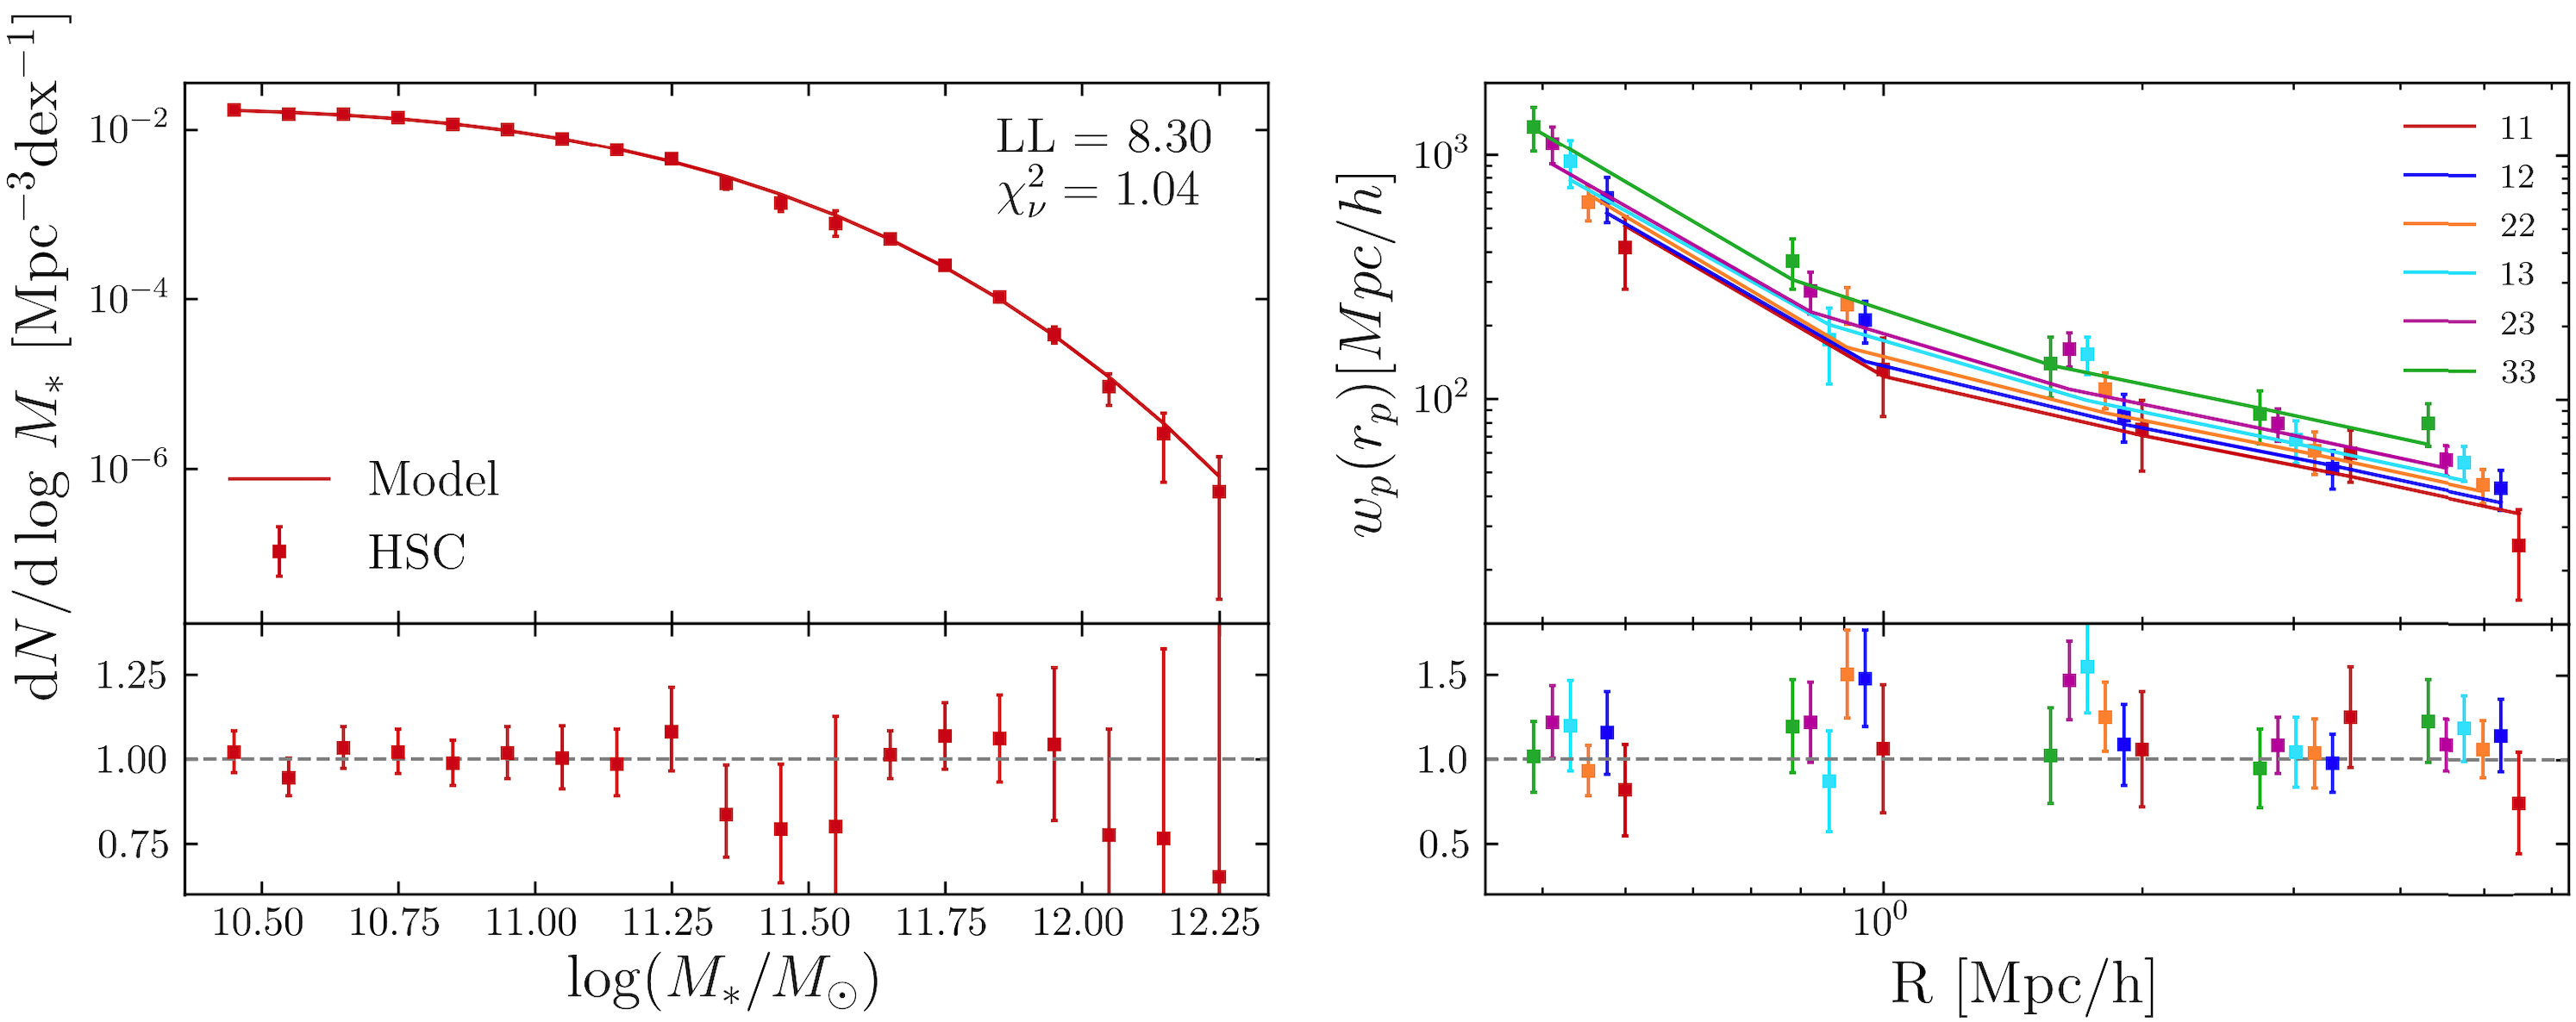
\includegraphics[width=\textwidth]{figure/mock_placeholder}
  \caption{\song{Placeholder} The best-fit mock matches both the SMF from HSC and PRIMUS (left)
    as well as the clustering from HSC. The mass bins for the clustering are [$11.5$, $11.55$,
    $11.7$, inf] and so e.g. "11" denotes the autocorrelation in the lowest mass bin and "13" the
    cross correlation between objects in the lowest and highest mass bins.}
  \label{fig:best_mock}
\end{figure*}
%% ---------------------------------------------------------------------------------------------- %%


%% ---------------------------------------------------------------------------------------------- %%
%% Scaling relation and scatters
%% ---------------------------------------------------------------------------------------------- %%
\subsection{Simple Scaling Relation Model}
    \label{sec:scaling}

We can model the effect on the DS profile of various amounts of scatter between a generic
observable, the log of which we denote as \obsSym{}, and the log of $\Mhalo$, denoted as $\mu$.
We assume that the relationship between halo mass and the observable is modeled by a power law
for the mean relation with lognormal scatter. This has been used for various observables, {\it
e.g.,\/} X-ray temperature \citet{Lieu2016}, K-band luminosity \citet{Ziparo2016}, and the
details of the statistics of this relation are described in, amongst others, \citet{Evrard2014,
Farahi2018}.

The relationship between \obsSym{} and $\mu$ will depend on the distribution of $\mu$ - this is
the halo mass function (HMF). To express the HMF over the full mass range, a functional form that
follows a power law at low masses with an exponential decline at high masses is generally used
\citep[\eg{}][]{Tinker2008}. However, as we are only interested in a narrow range at the high
mass end, we can approximate it as an exponential decline with some curvature.

\begin{equation}
    \hmf{} \equiv \frac{dn(\mu)}{d\mu{}}  = \exp \left(\beta_0 - \beta_1 \mu - \frac{\beta_2}{2} \mu^2 \right)
    \label{eq:quadratic_hmf}
\end{equation}

\noindent In practice, at the high mass end the mass function is decreasing ($\beta_1 > 0$) and
steepening ($\beta_2 > 0$).

We populate our simulation's halos with this generic observable,

\begin{equation}
    \obsSym = \mathcal{N}(\slope \mu + \intercept,\ \scatterObsSymMhalo)
    \label{eq:lognormal_obs_given_mhalo}
\end{equation}

However, while \scatterObsSymMhalo{} is physically meaningful and the number most often quoted
(\eg{} it is well known that $\scatterMstarx{cen} \sim 0.2$ dex) when comparing observables used
to select halos, it is the scatter in \Mhalo{} at a fixed value for the observable,
\scatterMhaloObsSym{}, that is important. We can compute the moments of $\mu | \obsSym$ as
follows.

We first note that the number of objects in a thin range of $\obsSym \in [\obsSym_1, \obsSym_2]$
is given by,

\begin{equation}
    N(\obsSym{}_1, \obsSym{}_2) \equiv \int_{\obsSym{}_1}^{\obsSym{}_2} \int_{-\infty}^{\infty} \hmf{} P(\obsSym{} | \mu) d\mu d\obsSym{}
\end{equation}


At fixed \obsSym{} we can therefore compute the expected $\mu$, and the scatter around it,

\begin{equation}
\begin{aligned}
    \langle \mu | \obsSym \rangle 
    &= \frac{1}{N(s_1, s_2)}
        \int_{-\infty}^{\infty} \hmf{} P(\obsSym{} | \mu) \mu d\mu \\
    &= \frac{\left( \frac{\obsSym- \intercept}{\slope} - \beta_1 \left(\frac{\scatterObsSymMhalo}{\slope}\right)^2 \right)}{ 1 + \beta_2 \left(\frac{\scatterObsSymMhalo}{\slope}\right)^2}
    \label{eq:mean_of_mu}
\end{aligned}
\end{equation}

\noindent The three components of $\langle \mu | \obsSym \rangle$ are: 
\begin{enumerate}
	
    \item The relation between the observable and halo mass, $(\obsSym- \intercept) / \slope$.

    \item A shift due to the Eddington bias caused by the linear slope of the HMF, $-\beta_1
        (\scatterObsSymMhalo / \slope)^2$. In the case of $\beta_1 > 0$, this shift is to lower $\mu$ as
        there are more low $\mu$ objects that can be up-scattered into the selection than can be
        down-scattered.

    \item A second shift due to excess Eddington bias caused by the curvature of the HMF, $(1 +
        \beta_2 (\frac{\scatterObsSymMhalo}{\slope})^2)^{-1}$. Again, $\beta_2 > 0$ results in more low
        $\mu$ objects and thus a shift to lower $\mu$.
	
\end{enumerate}

Similarly, the scatter in $\mu$ at fixed $\obsSym$,

\begin{equation}
\begin{aligned}
    \scatterMhaloObsSym{} 
    &= \frac{1}{N(s_1, s_2)}
        \int_{-\infty}^{\infty} \hmf{} P(\obsSym{} | \mu) ( \mu  - \langle \mu \rangle )^2 d\mu \\
	&= \frac{\scatterObsSymMhalo}{\sqrt{\beta_2 \scatterObsSymMhalo^2 + \slope^2}}
    \label{eq:scatter_of_mu}
\end{aligned}
\end{equation}

\noindent which, in the case of a power law mass function, reduces to the commonly seen
$\scatterObsSymMhalo / \slope$. The positive $\beta_2$ of the HMF decreases this scatter.
Finally, higher moments show that $P(\mu | s)$ is Gaussian, as there is no skew or excess
kurtosis.

These results are summarized in the left panel of Figure \ref{fig:theory} where we simulate the
HMF and the theoretical observable \obsSym{}. We show that the resulting distributions are
consistent with the results shown here.

This theoretical understanding of the moments on $\mu | \obsSym$ shows us what range of slope and
scatter we need to generate \dsigma{} profiles for. While naively this is a 2 dimensional
problem, \ref{eq:scatter_of_mu} shows that it can be reduced to a single dimension where
\scatterMhaloObsSym{} is a function of the ratio between slope and scatter. This is obvious in
the case where $\beta_2 = 0$ but still true in the curved case,

\begin{equation}
    \scatterMhaloObsSym{} 
    	= \frac{\scatterObsSymMhalo}{\sqrt{\beta_2 \scatterObsSymMhalo^2 + \slope^2}}
        = \left(\beta_2 + (\frac{\slope}{\scatterObsSymMhalo})^2\right)^{-1/2}
    \label{eq:ratio_is_what_matters}
\end{equation}

This is shown in the right panel of Figure \ref{fig:theory}. For a variety of observables with a
range of $\alpha$ and \scatterObsSymMhalo{}, but with the same ratio $\alpha /
\scatterObsSymMhalo$, and therefore the same \scatterMhaloObsSym{}, the DS is identical.
Therefore, in order to compare the DS from a range of observables with different slope/scatter
compared to have mass, we can fix one parameter ($\alpha = 1$) and vary the other
($\scatterObsSymMhalo$) to achieve the goal \scatterMhaloObsSym{} in the number density bins
discussed in \ref{sec:topn_intro}. In practice, rather than predict the \scatterMhaloObsSym{}
using \ref{eq:scatter_of_mu} (which requires fitting for $\beta_2$ at that point in the HMF), we
instead binary search for the desired \scatterMhaloObsSym{} by iteratively choosing a
\scatterObsSymMhalo{} to populate the halos with, and then fitting a linear $\mu | \obsSym$ to
the relation in the given halo mass bin. The results of this process are shown in \ref{fig:mdpl2}
where we predict DS profiles as a function of \scatterMhaloObsSym{} for each of the number
density bins. We will compare these theoretical predicts to the observables to estimate their
\scatterMhaloObsSym{}.

%% ---------------------------------------------------------------------------------------------- %%
%% Model used in comparison
%% ---------------------------------------------------------------------------------------------- %%
\subsection{Model Calibrated to Match HSC}
    \label{sec:halo_model}

\todo{Placeholder: Need to be updated}
\textcolor{blue}{Chris to write this up and compute}

While the simple scaling relation model presented above is useful to predict the effects of
scatter between an observable and halo mass on the lensing signal, a more detailed model of the
galaxy halo connection is needed to compare with specific model of M100. To make comparisons the
HSC observations and theory, we need to populate the simulation with realistic galaxies. This
process will be described in more detail in (Bradshaw et. al. 2020 (in prep.)) but we summarize
it here.

To do this, we use the 1Gpc MultiDark-Planck simulation. We populate galaxies using an abundance
matching model based on the \citet{Lehmann2017} $\alpha$ model. This model marginalizes over the
choice of the halo property to abundance match on. In this analysis, we use the mock that best
fits the HSC high mass clustering, the auto- and cross-correlation of $\omega_p$ in bins of
stellar mass [$11.5$, $11.55$, $11.7$, inf], and the combination of the SMF from HSC and PRIMUS.
We use the HSC SMF in the mass regime that is complete ($> 11.5$) and PRIMUS for lower masses
($10.5 - 11.5$).

The best-fit mock is able to reproduce the mass function and clustering statistics of HSC as
shown in \ref{fig:best_mock}.

%% ---------------------------------------------------------------------------------------------- %%
%% Figure: Definition of richness and number density bins.
%% ---------------------------------------------------------------------------------------------- %%
  \begin{figure*}
      \centering 
      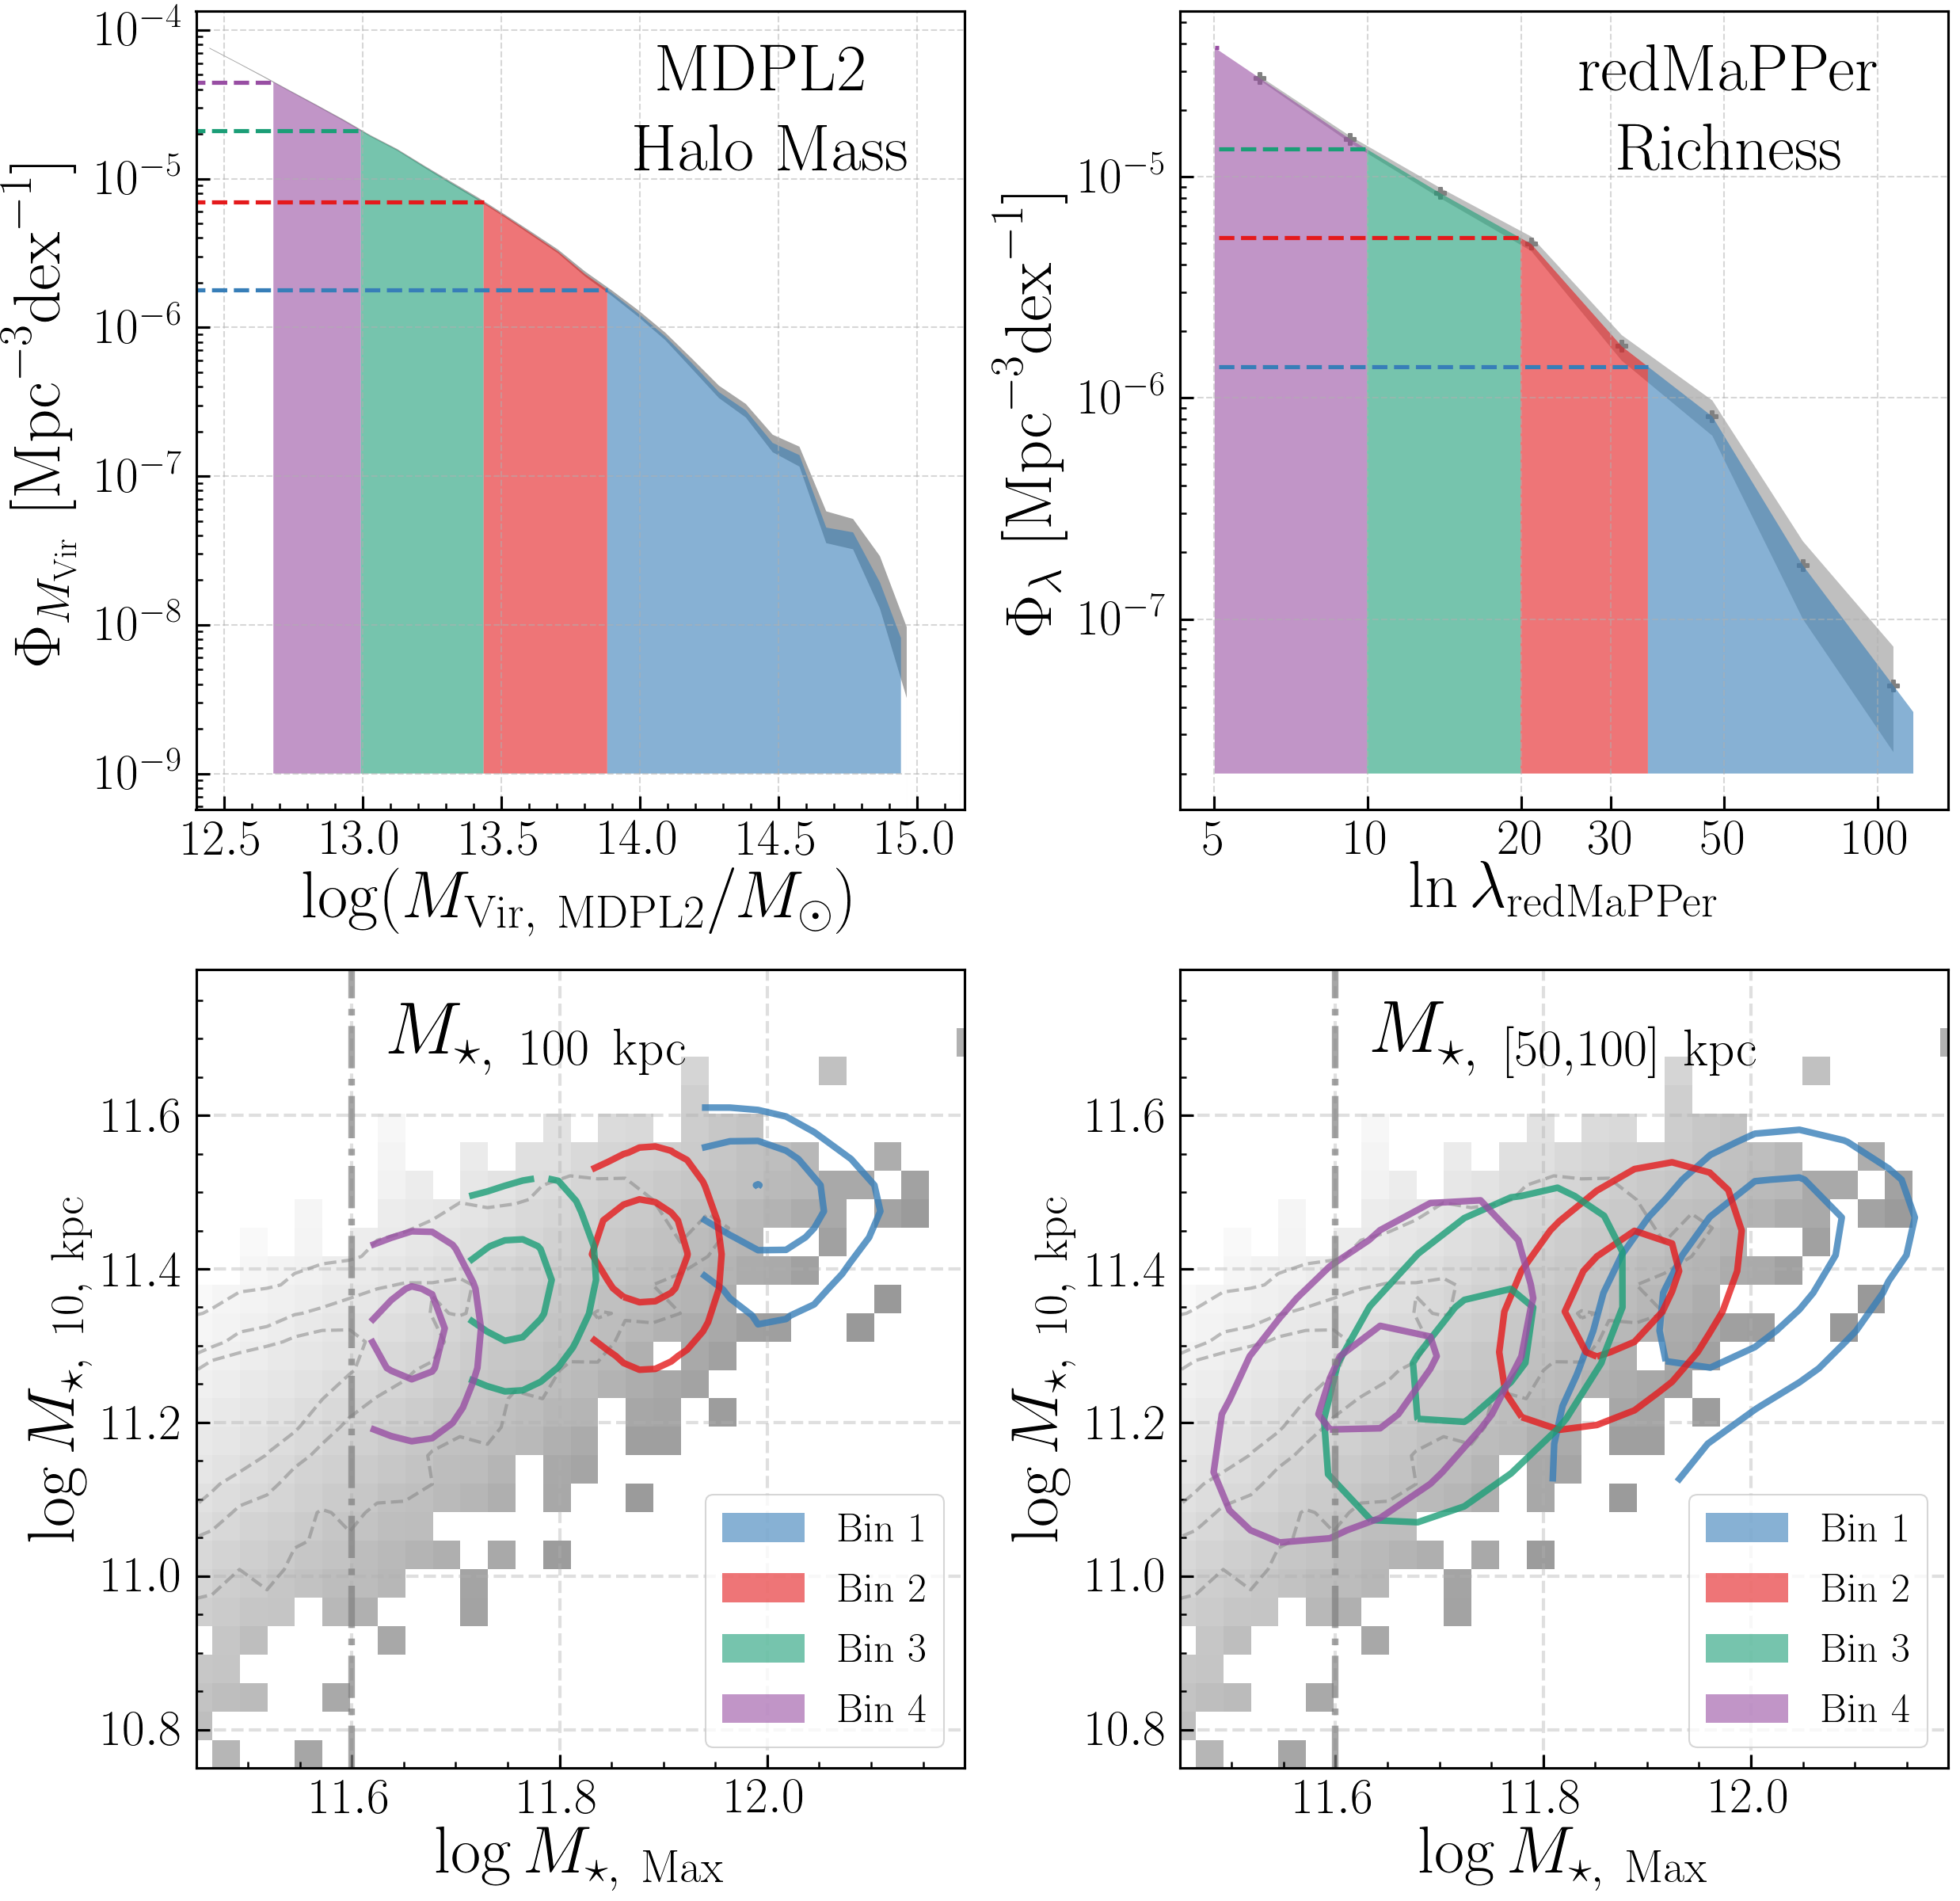
\includegraphics[width=\textwidth]{figure/topn_bins}
      \caption{The four bins used for our "top-N" tests. The left panel displays bins in
        $\lambda$, the middle panel displays bins in \mmax{}, and the right panel displays bins in
        $M_{\rm vir,\ ASAP}$. Bins are defined at fixed number density. \alexie{Add a table for
        each of the quantities with the edges of the bin and the mean bin. This can be two panels.
        The phi one on the left and the two parameter cut on the right to highlight why samples
        can be different}}
      \label{fig:density_bins}
  \end{figure*}
%% ---------------------------------------------------------------------------------------------- %%

%% ---------------------------------------------------------------------------------------------- %%
%% Figure: DSigma profiles from MDPL2 and the impacts of scatter on DSigma profile and 
%%         halo mass distribution
%% ---------------------------------------------------------------------------------------------- %%
  \begin{figure*}
      \centering 
      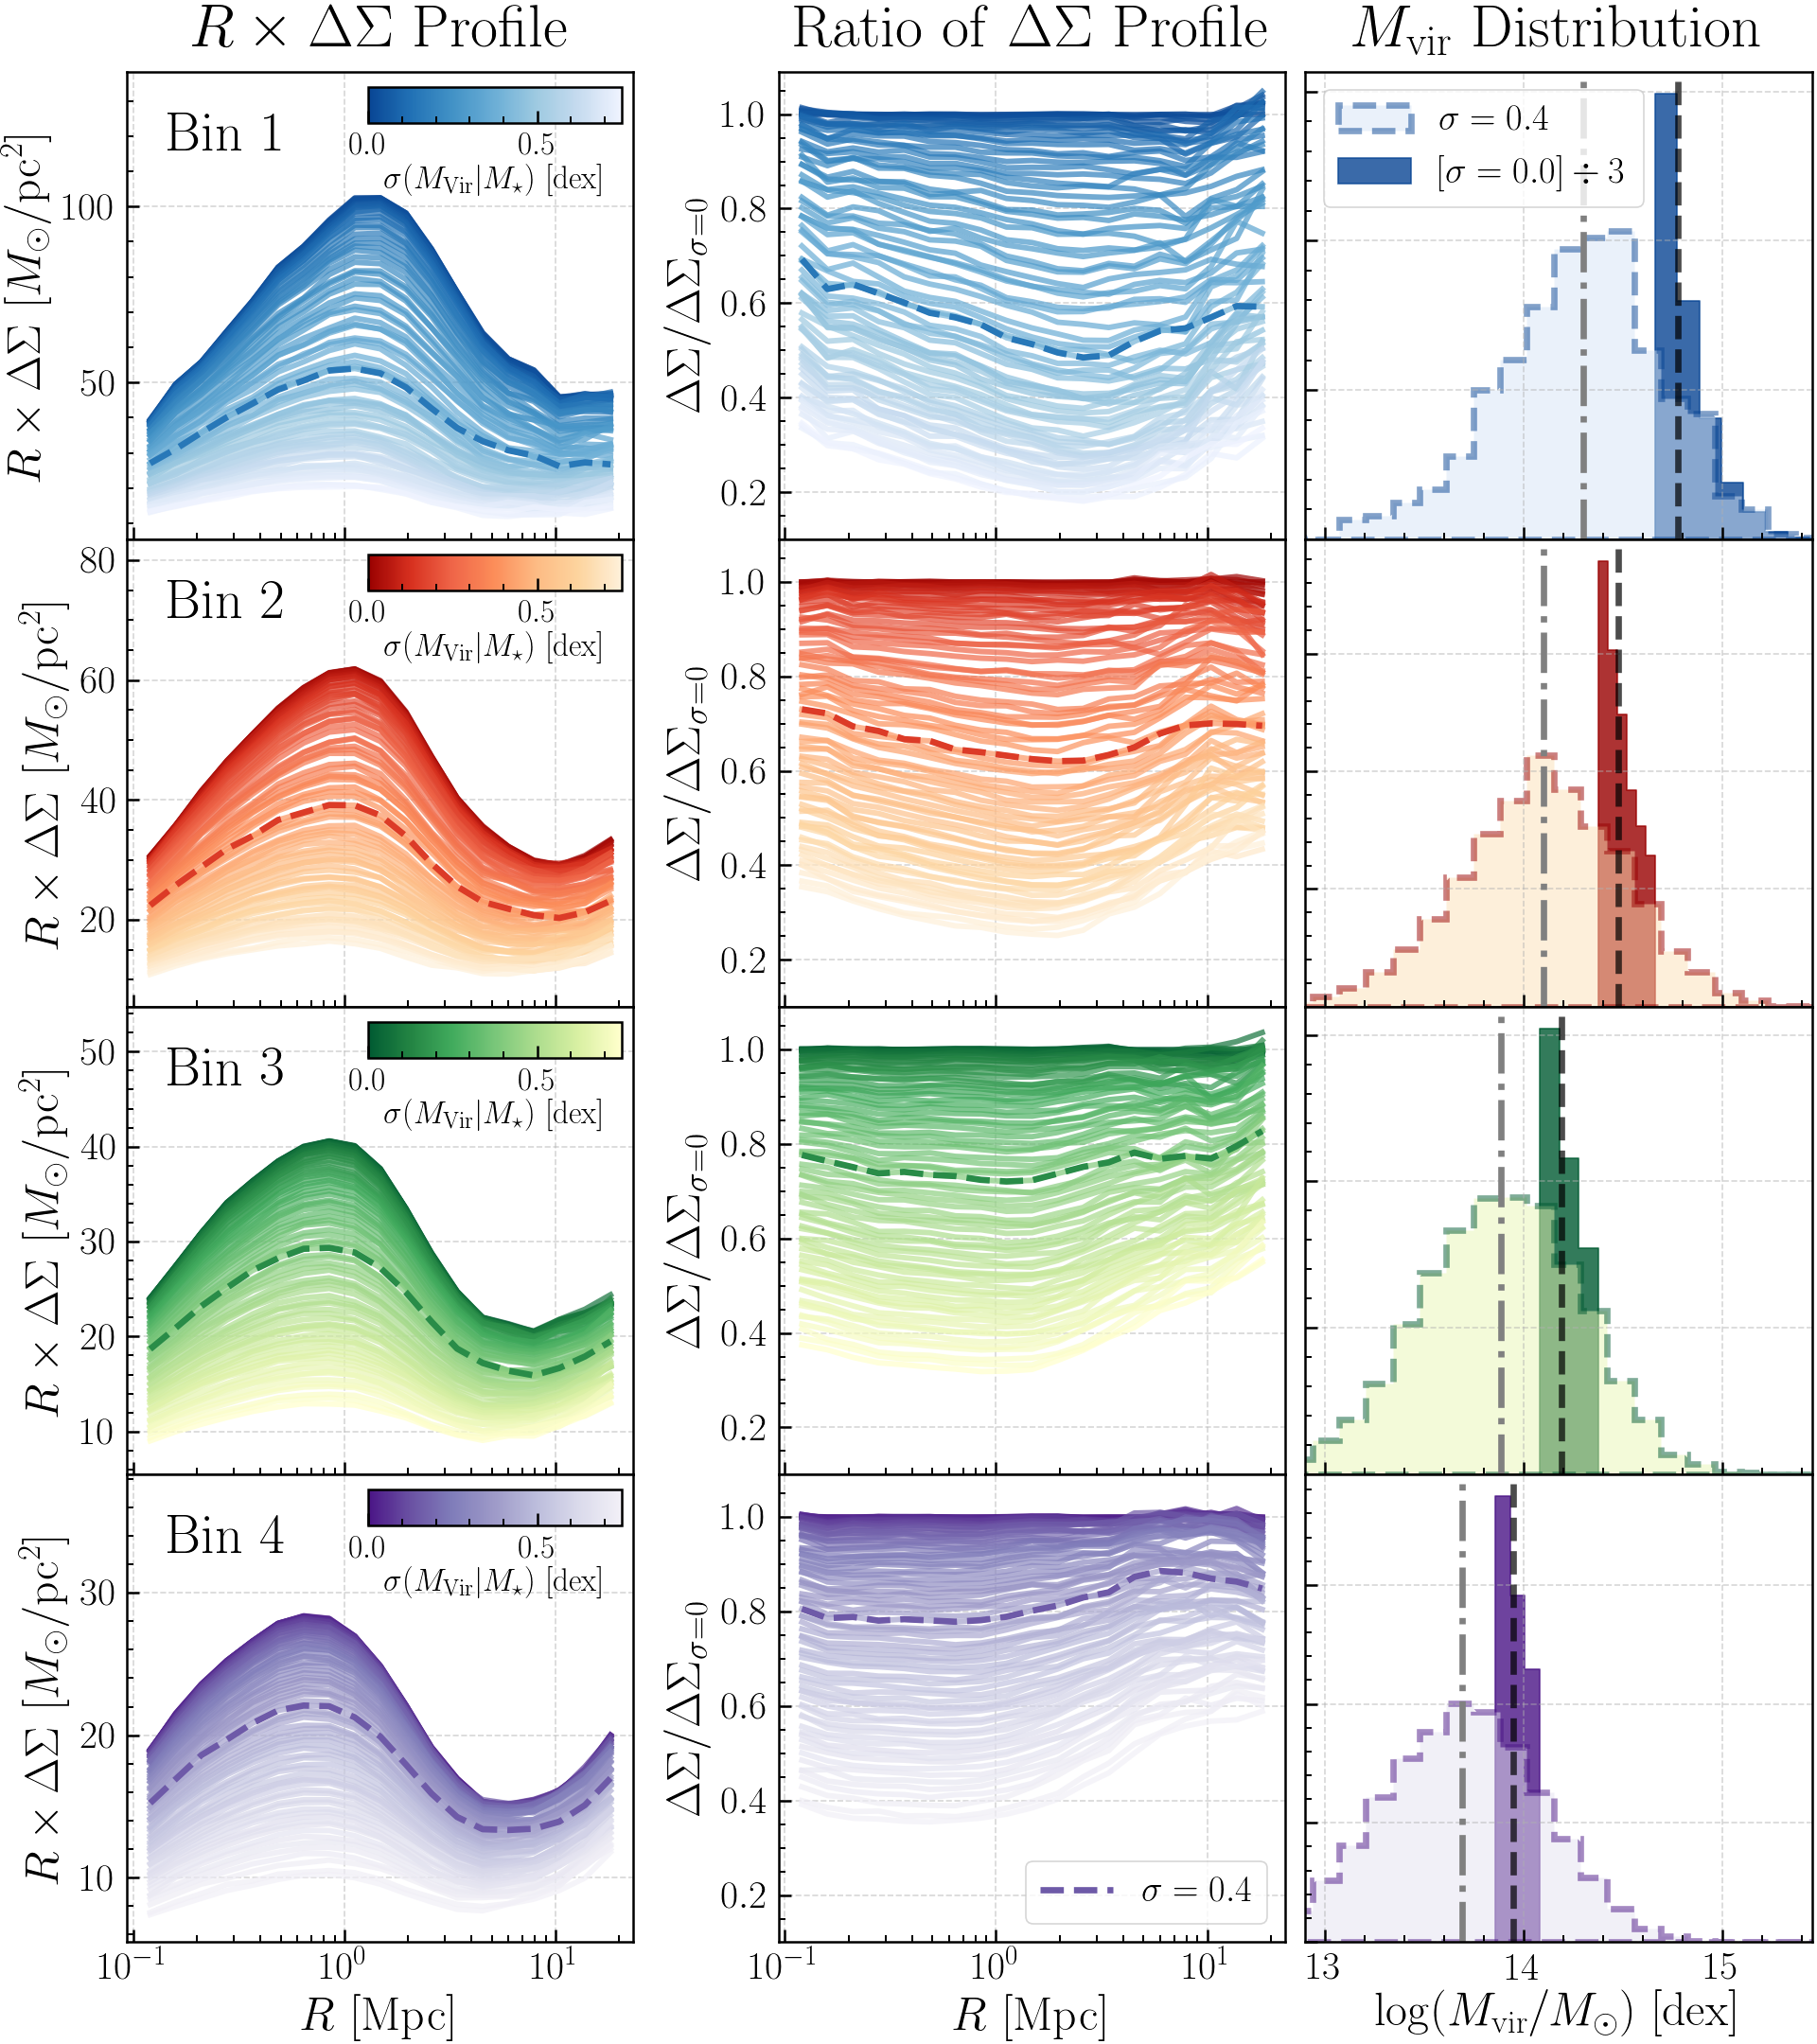
\includegraphics[width=\textwidth]{figure/topn_mdpl2_dsigma}
      \caption{Impact of scatter in the mass-observable relation on $\Delta\Sigma$. Left: the
        $\Delta\Sigma$ profiles for $0<\sigma_{Mvir|obs}<2$. Middle: ratio of $\Delta\Sigma$ with
        non zero scatter to $\Delta\Sigma$ when $0<\sigma_{Mvir|obs}=0$. Right: halo mass
        histograms for bin 1 ($\overline(n)=x$) and bin 2 ($\overline(n)=x$).} \label{fig:mdpl2}
  \end{figure*}
%% ---------------------------------------------------------------------------------------------- %%

%% ---------------------------------------------------------------------------------------------- %%
%% Table.1 
%% ---------------------------------------------------------------------------------------------- %%
%\clearpage
\begin{table*}
\resizebox{0.7\textwidth}{!}{%
\small
\begin{tabular}{|c|cccc|}
\hline
\rowcolor[HTML]{d8dcd6} Property   & Bin 1   & Bin 2   & Bin 3  & Bin 4 \\ \hhline{|=====|}

$N_{\rm Sample}$     &   50  &  197  &  662  &  1165  \\  

$\log_{10} M_{\rm vir,\ \rm MDPL2}$  & [14.66, 15.55] & [14.38, 14.66) & [14.08, 14.38) & [13.86, 14.08) \\

$n(>M_{\rm vir})$  & $5.11\times 10^{-7}$ & $2.52\times 10^{-6}$ & $9.29\times 10^{-6}$ & $2.12\times 10^{-5}$ \\ \hhline{|=====|}

\multirow{2}{*}{$\lambda_{\rm redMaPPer}$}  &  [35, 120] &  [20, 35)  & [10, 20) &  [6, 10)  \\
& \sigmvir{}$=0.27\pm0.02$ & $0.38\pm0.02$ & $0.39\pm0.02$ & $0.58\pm0.02$ \\ \hline
                                            
\multirow{2}{*}{$N_{\rm CAMIRA}$}  &  [35, 75) & [21, 35) & [12, 21) &  \\
& \sigmvir{}$=0.30\pm0.03$ & $0.36\pm0.01$ & $0.50\pm0.02$ & {} \\ \hhline{|=====|}

\multirow{2}{*}{$\log_{10} M_{\star, \rm CModel}$}   & [11.88, 12.19] & [11.77, 11.88) & [11.67, 11.77) & [11.60, 11.67) \\ 
& \sigmvir{}$=0.60\pm0.04$ & $0.64\pm0.04$ & $0.87\pm0.06$ & $0.82\pm0.03$ \\ \hline

\multirow{2}{*}{$\log_{10} M_{\star, 30\ \rm kpc}$} & [11.77, 12.00] & [11.69, 11.77) & [11.61, 11.70) & [11.53, 11.61) \\ 
& \sigmvir{}$=0.52\pm0.04$ & $0.57\pm0.03$ & $0.61\pm0.03$ & $0.61\pm0.02$ \\ \hline

\multirow{2}{*}{$\log_{10} M_{\star, 50\ \rm kpc}$} & [11.86, 12.10] & [11.76, 11.86) & [11.66, 11.76) & [11.58, 11.66) \\ 
& \sigmvir{}$=0.46\pm0.04$ & $0.53\pm0.03$ & $0.59\pm0.02$ & $0.61\pm0.02$ \\ \hline

\multirow{2}{*}{$\log_{10} M_{\star, 100\ \rm kpc}$} & [11.93, 12.18] & [11.83, 11.93) & [11.71, 11.83) & [11.63, 11.71) \\ 
& \sigmvir{}$=0.38\pm0.02$ & $0.51\pm0.02$ & $0.56\pm0.02$ & $0.60\pm0.02$ \\ \hline

\multirow{2}{*}{$\log_{10} M_{\star, 150\ \rm kpc}$} & [11.96, 12.21] & [11.85, 11.96) & [11.73, 11.85) & [11.64, 11.73)  \\ 
& \sigmvir{}$=0.37\pm0.03$ & $0.47\pm0.03$ & $0.56\pm0.02$ & $0.57\pm0.03$ \\ \hhline{|=====|}

\multirow{2}{*}{$\log_{10} M_{\star, [50, 100]}$} & [11.20, 11.60] & [11.00, 11.20) & [10.80, 11.00) & [10.63, 11.00)  \\ 
& \sigmvir{}$=0.36\pm0.02$ & $0.43\pm0.02$ & $0.44\pm0.02$ & $0.48\pm0.02$ \\ \hline

\multirow{2}{*}{$\log_{10} M_{\rm Vir,\ ASAP}$} & [14.45, 15.28] & [14.09, 14.45) & [13.80, 14.11) & [13.60, 13.80)  \\ 
& \sigmvir{}$=0.38\pm0.03$ & $0.44\pm0.02$ & $0.48\pm0.02$ & $0.56\pm0.02$ \\ \hline

\end{tabular}%
}
\caption{
	Summary of results from the \topn{} test results in four number density bins. 
	The first three rows summarize the basic properties of each bin.
	$N_{\rm sample}$ is the number of HSC galaxies in each bin. 
	$\log_{10}M_{\rm vir, MDPL2}$ shows the corresponding halo mass range in this number density bin
	based on the \mdpl2{} simulation. 
	This is the \mvir{} range for an ideal (zero scatter) \topn{} selection.
	$n(>M_{\rm Vir})$ is the volume number density of halos above the lower-\mvir{} threshold.
	Subsequent rows contain the key results for different halo mass proxies. 
	The first row shows the range of the observed properties in the four bins.  The second row shows
	the best--fit scatter of \mvir{} at fixed observable ($\sigma_{\mathcal{M}|\mathcal{O}}$) of
	\mvir{} in each bin along with its uncertainty.
	For a complete summary table of all the properties we tested, please see this \texttt{Jupyter} notebook \href{https://github.com/dr-guangtou/jianbing/blob/master/notebooks/topn_result_summary.ipynb}{\faGithub} 
	}
\label{tab:summary}
\end{table*}
%\clearpage
%% ---------------------------------------------------------------------------------------------- %%

%% ---------------------------------------------------------------------------------------------- %%
%% Main Results
%% ---------------------------------------------------------------------------------------------- %%
\section{Results}
    \label{sec:result}

  Now we summarize the key results from the ``Top N'' tests

%% ---------------------------------------------------------------------------------------------- %%
%% Impact of satellite galaxies 
%% ---------------------------------------------------------------------------------------------- %%
\subsection{Impact of Satellites}
    \label{sec:satellite}

    Contaminations of satellite galaxies is the key systematic issue when using \mstar{} of 
    a single galaxy as \mvir{} tracer.

Figure \ref{fig:satellite} show the impact of satellites. Describe here.

%% ---------------------------------------------------------------------------------------------- %%
%% Figure: Impact of satellites on the M100kpc selected DSigma profiles
%% ---------------------------------------------------------------------------------------------- %%
  \begin{figure}
      \centering 
      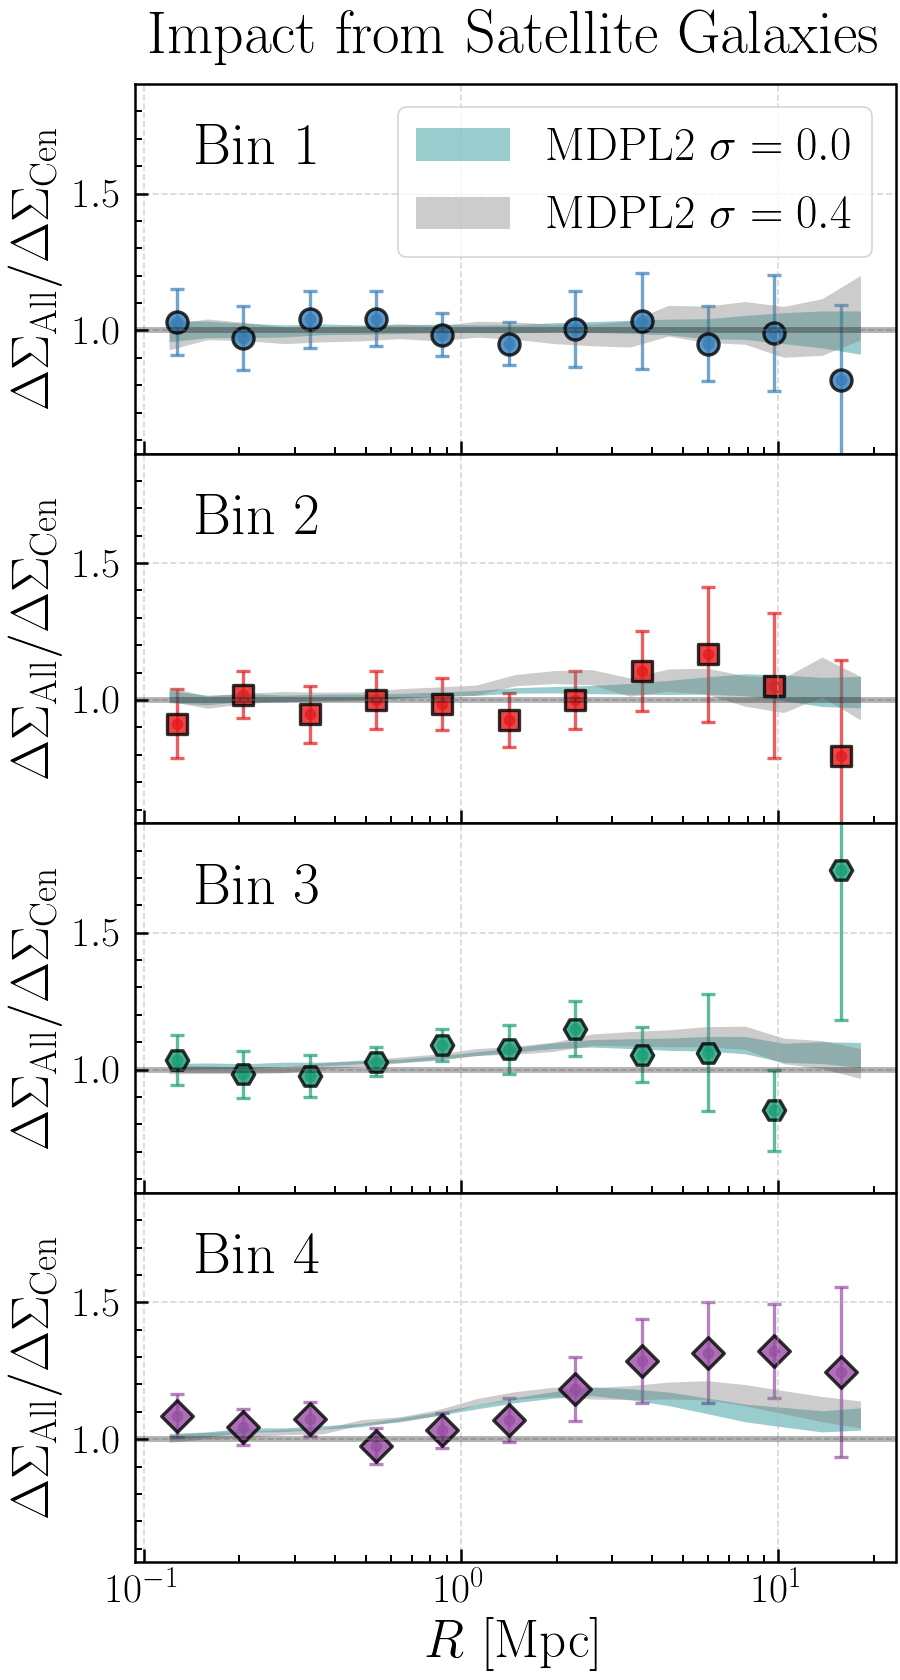
\includegraphics[width=0.49\textwidth]{figure/dsigma_sat_ratio}
      \caption{
          \todo{Impact of satellites on the M100kpc selected \dsigma{} profiles}
          }
      \label{fig:satellite}
  \end{figure}
%% ---------------------------------------------------------------------------------------------- %%


%% ---------------------------------------------------------------------------------------------- %%
%% Poor performance of CModel stellar mass 
%% ---------------------------------------------------------------------------------------------- %%
\subsection{Performance of \mcmodel{}}

\plan{CModel is terrible, not good, very bad}

%% ---------------------------------------------------------------------------------------------- %%
%% Performance of outer envelope mass
%% ---------------------------------------------------------------------------------------------- %%
\subsection{Performance of the \mstar{} of outer enevelope}

\plan{We are surprised by the performance of outer envelope mass}

%% ---------------------------------------------------------------------------------------------- %%
%% General trends of scatters
%% ---------------------------------------------------------------------------------------------- %%
\subsection{Performance of the \mstar{} of outer enevelope}

\plan{Remind people that the scatter here is scatter of halo mass, is for each bin, and is 
    only useful for relative comparison.}

%% ---------------------------------------------------------------------------------------------- %%
%% Figure: Summary of HSC DSigma profiles and the distributions over the aperture stellar 
%%         mass plane.
%% ---------------------------------------------------------------------------------------------- %%
%  \begin{figure*}
%      \centering 
%      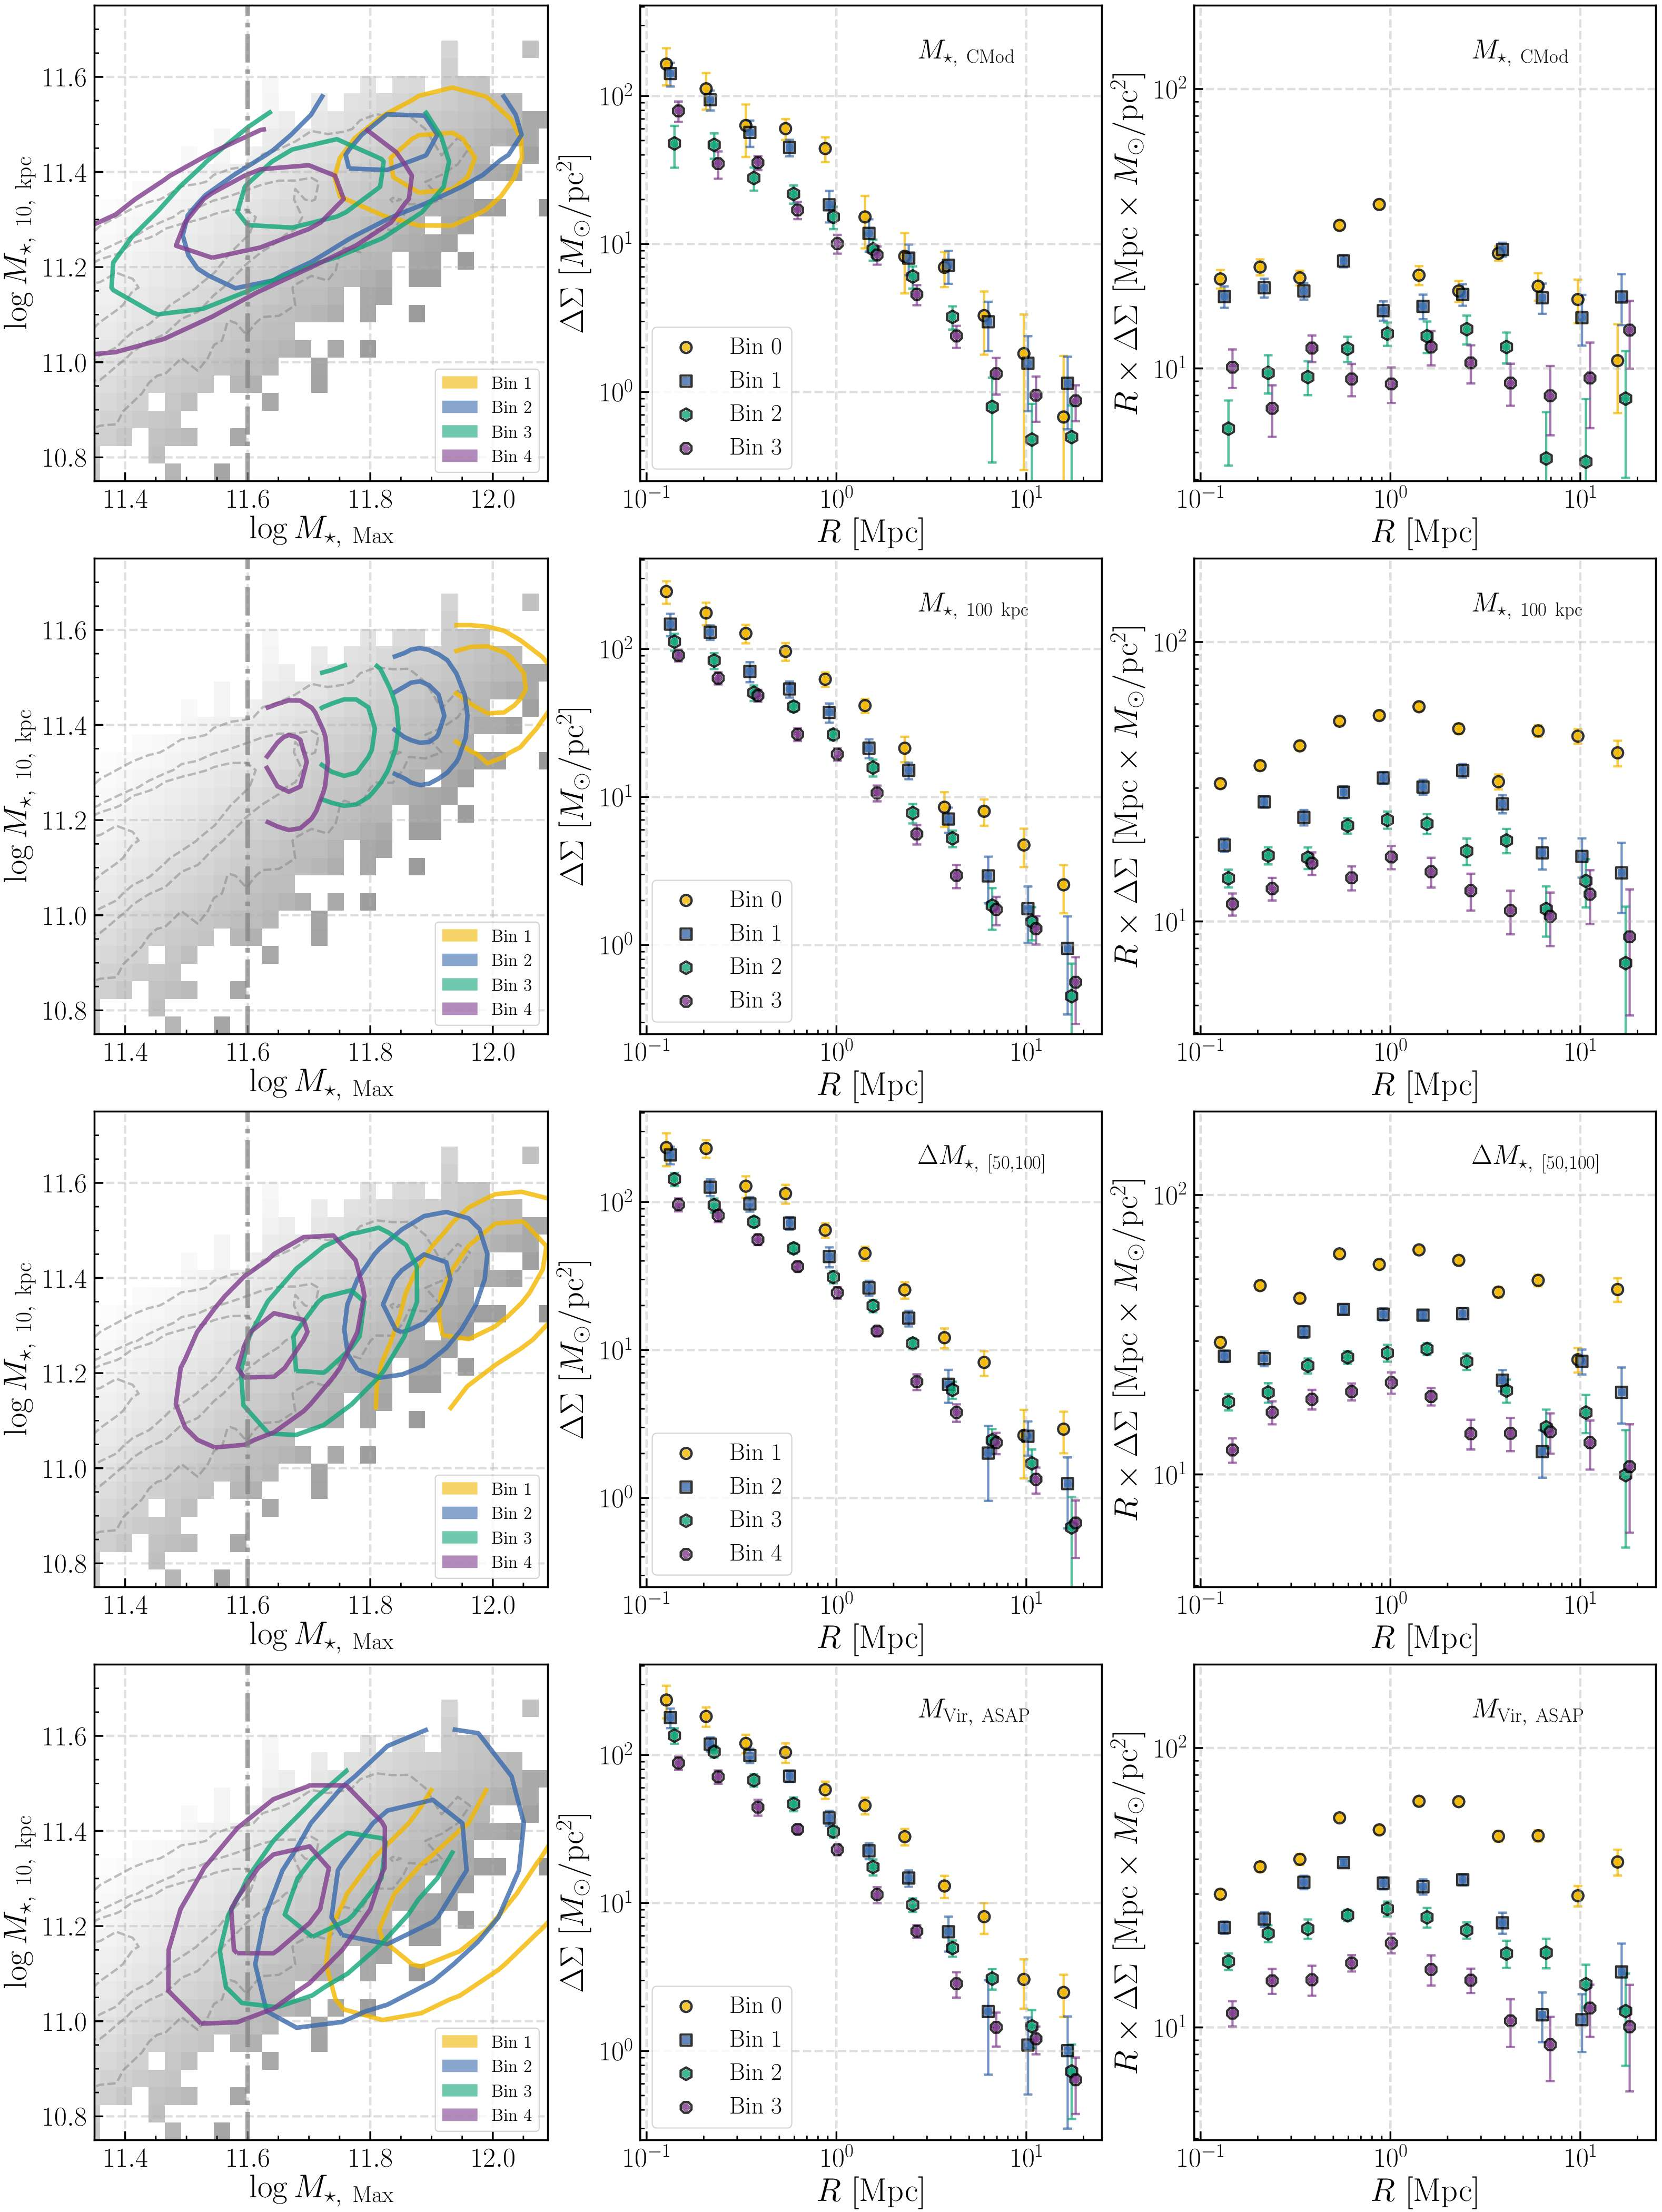
\includegraphics[width=15.5cm]{fig/small/topn_dsigma_summary}
%      \caption{
%          \todo{Summary of the \dsigma{} profiles from HSC using different tracers.
%          		Also highlight their distributions over the \mmax{}-\minn{} plane. \alexie{replace the left hand side with histograms of halo mass. }}
%          }
%      \label{fig:hsc}
%  \end{figure*}
%% ---------------------------------------------------------------------------------------------- %%
       
%% ---------------------------------------------------------------------------------------------- %%
%% Trends with scatter
%% ---------------------------------------------------------------------------------------------- %%
\subsection{Scatter in Halo Mass at Fixed Observable}

%Figure \ref{fig:scatter1} and \ref{fig:scatter2} show the scatter in halo mass at fixed observable.

%% ---------------------------------------------------------------------------------------------- %%
%% Figure: Comparisons of scatters: different tracers and aperture masses
%% ---------------------------------------------------------------------------------------------- %%
  \begin{figure*}
      \centering 
      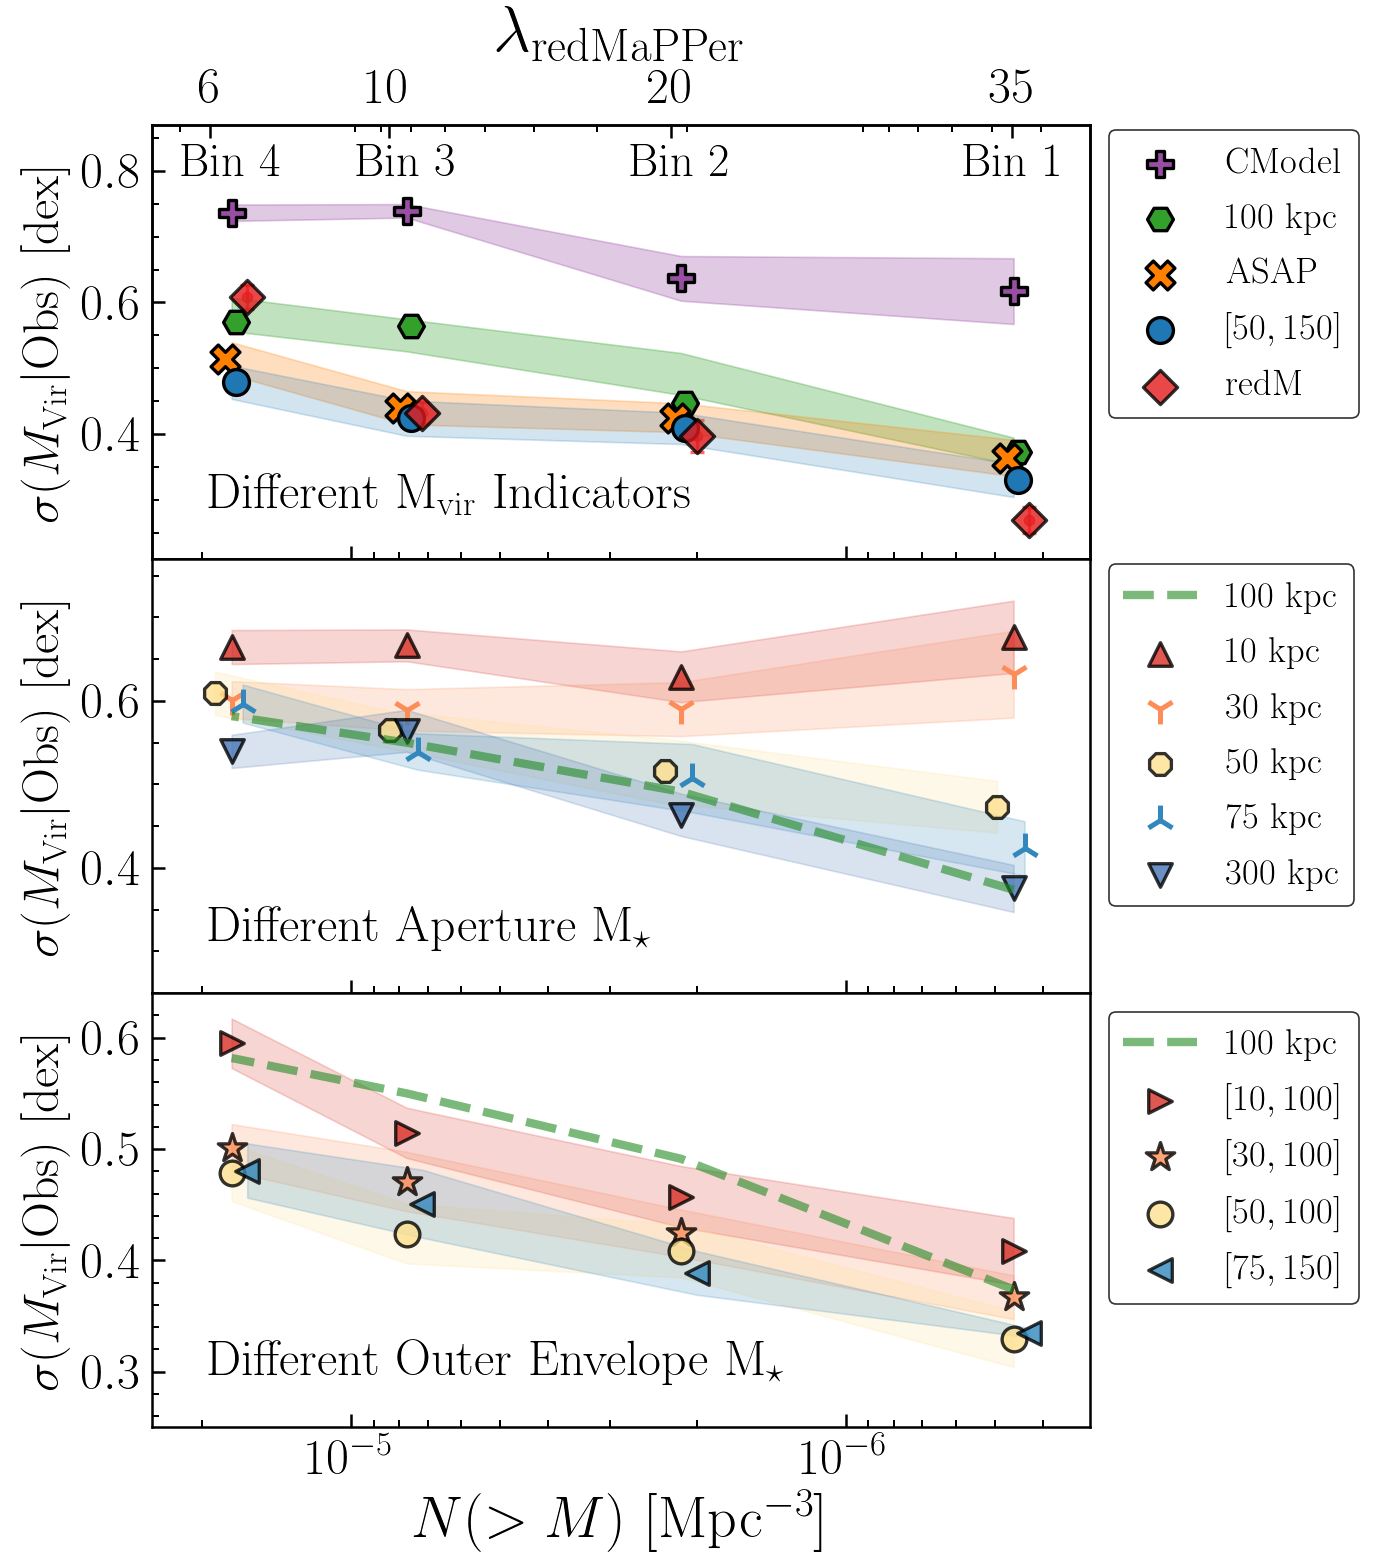
\includegraphics[width=0.85\textwidth]{figure/topn_sigma_trend_sum}
      \caption{
          \todo{Comparisons of scatters: different tracers and aperture masses. \alexie{Can you make the colors more bold here? These colors are kinnda pale. We want something bold and flashy.}}
          }
      \label{fig:scatter1}
  \end{figure*}
%% ---------------------------------------------------------------------------------------------- %%

%% ---------------------------------------------------------------------------------------------- %%
%% Comparison with richness selected galaxies
%% ---------------------------------------------------------------------------------------------- %%
\subsection{Analysis of the Shape of $\Delta\Sigma$}

Here we consider specifically the shape of $\Delta\Sigma$. 

%The main figures are \ref{fig:m100} and \ref{fig:mout}. Discuss the best fits and the presence of the bump.

%% ---------------------------------------------------------------------------------------------- %%
%% Figure: Compare M100kpc mass and CModel mass
%% ---------------------------------------------------------------------------------------------- %%
  \begin{figure*}
      \centering 
      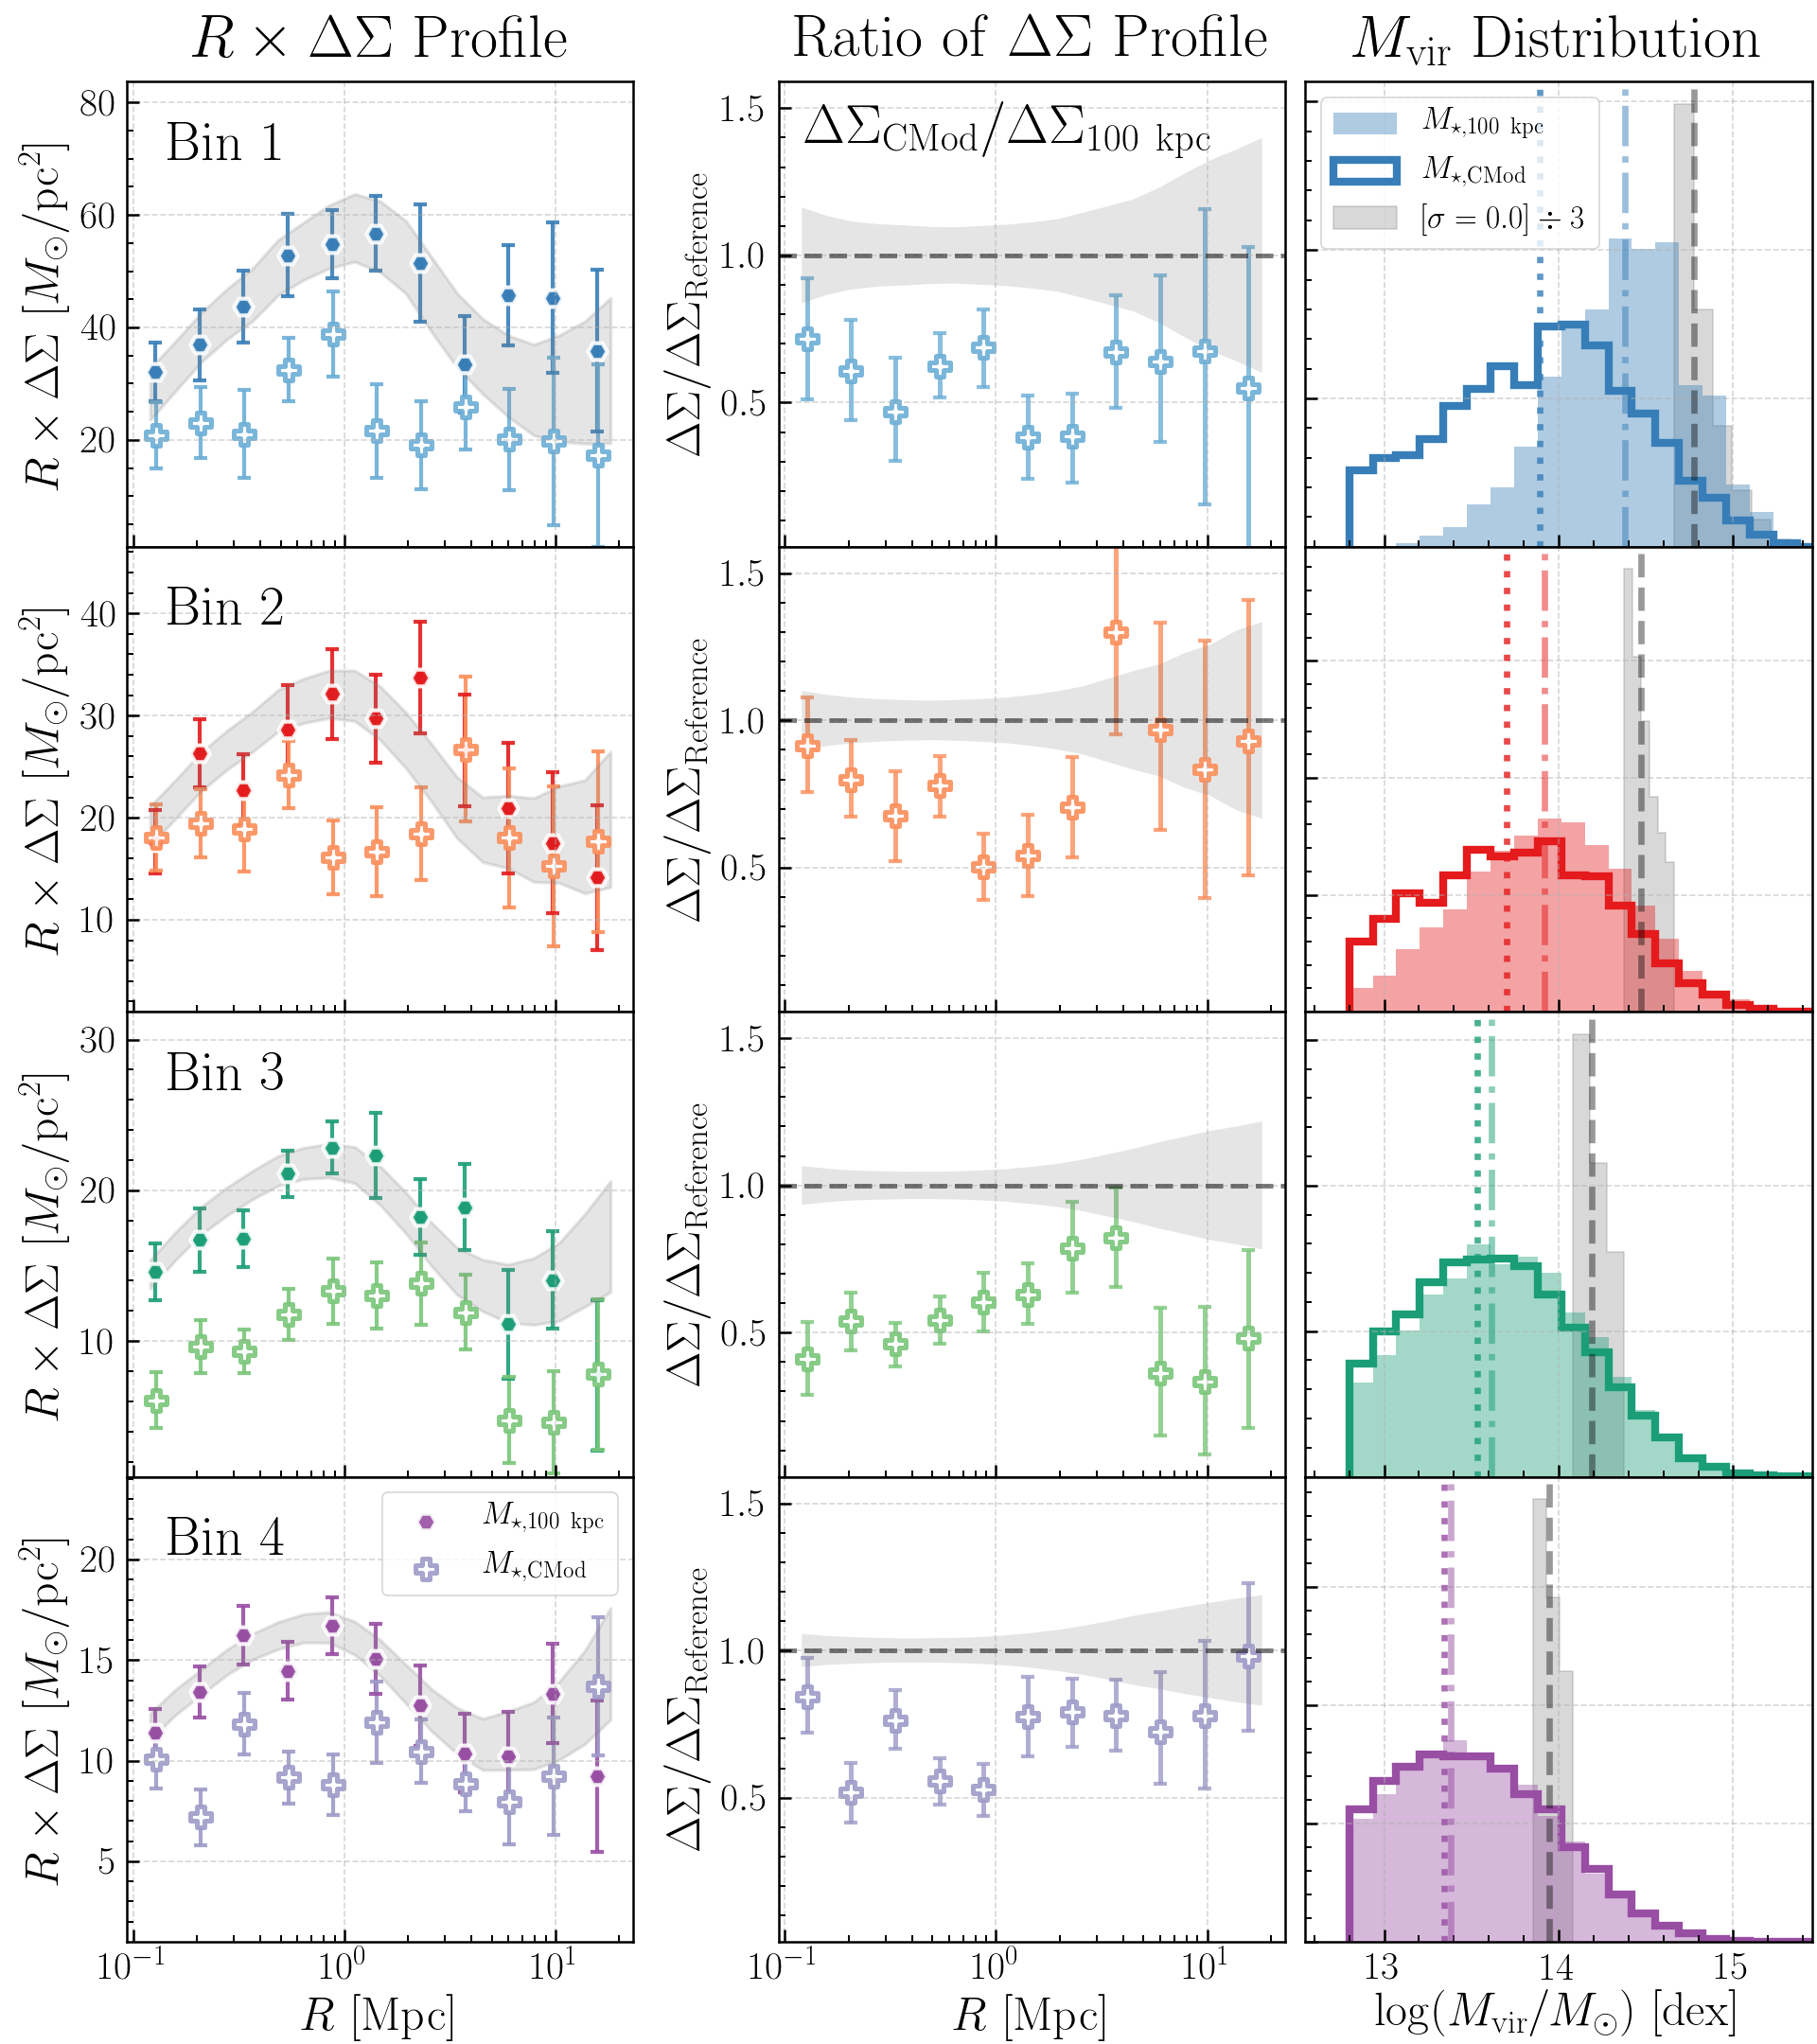
\includegraphics[width=\textwidth]{figure/topn_dsigma_m100_cmod_compare}
      \caption{
          \todo{Compare M100kpc and CModel mass}
          }
      \label{fig:m100_cmod}
  \end{figure*}
%% ---------------------------------------------------------------------------------------------- %%

%% ---------------------------------------------------------------------------------------------- %%
%% Figure: Compare 50-100 kpc outer envelope mass and 100 kpc mass
%% ---------------------------------------------------------------------------------------------- %%
  \begin{figure*}
      \centering
      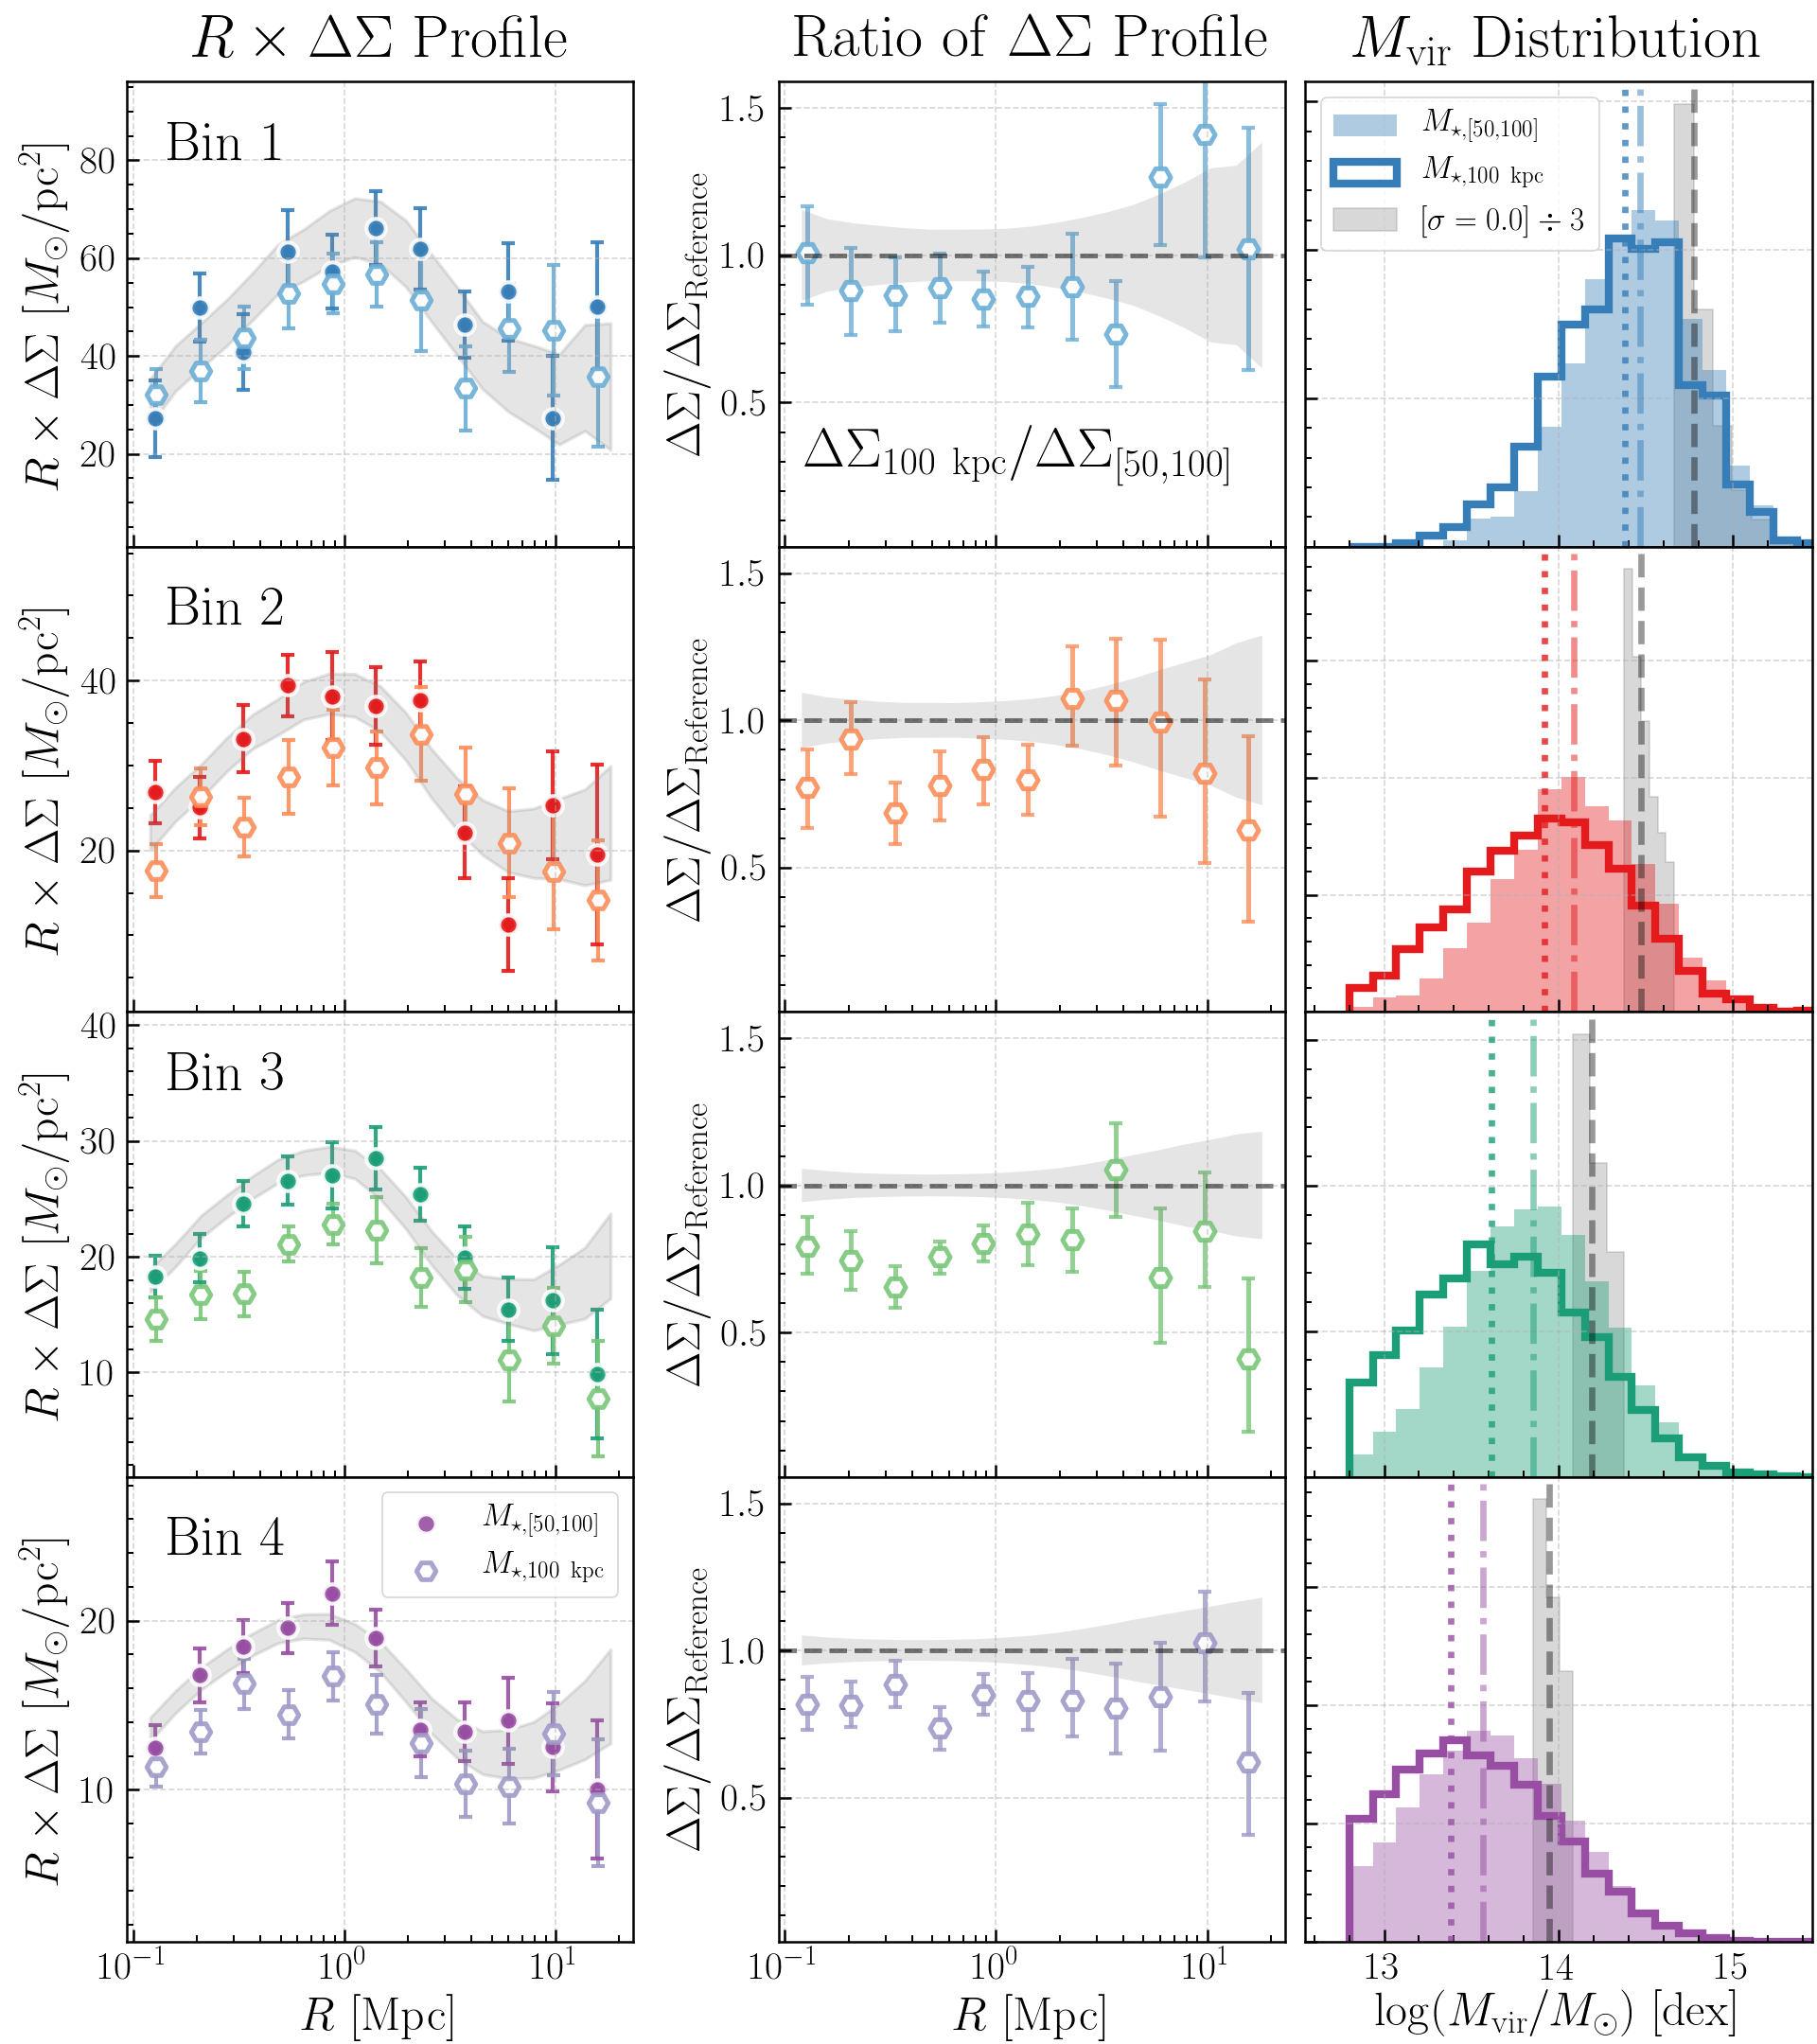
\includegraphics[width=\textwidth]{figure/topn_dsigma_m100_mout_compare}
      \caption{
          \todo{Compare 50-100 kpc outer envelope mass and 100 kpc mass}
          }
      \label{fig:m100_mout}
  \end{figure*}
%% ---------------------------------------------------------------------------------------------- %%

%% ---------------------------------------------------------------------------------------------- %%
%% Figure: Compare 50-100 kpc outer envelope mass and richness selected clusters
%% ---------------------------------------------------------------------------------------------- %%
  \begin{figure*}
      \centering
      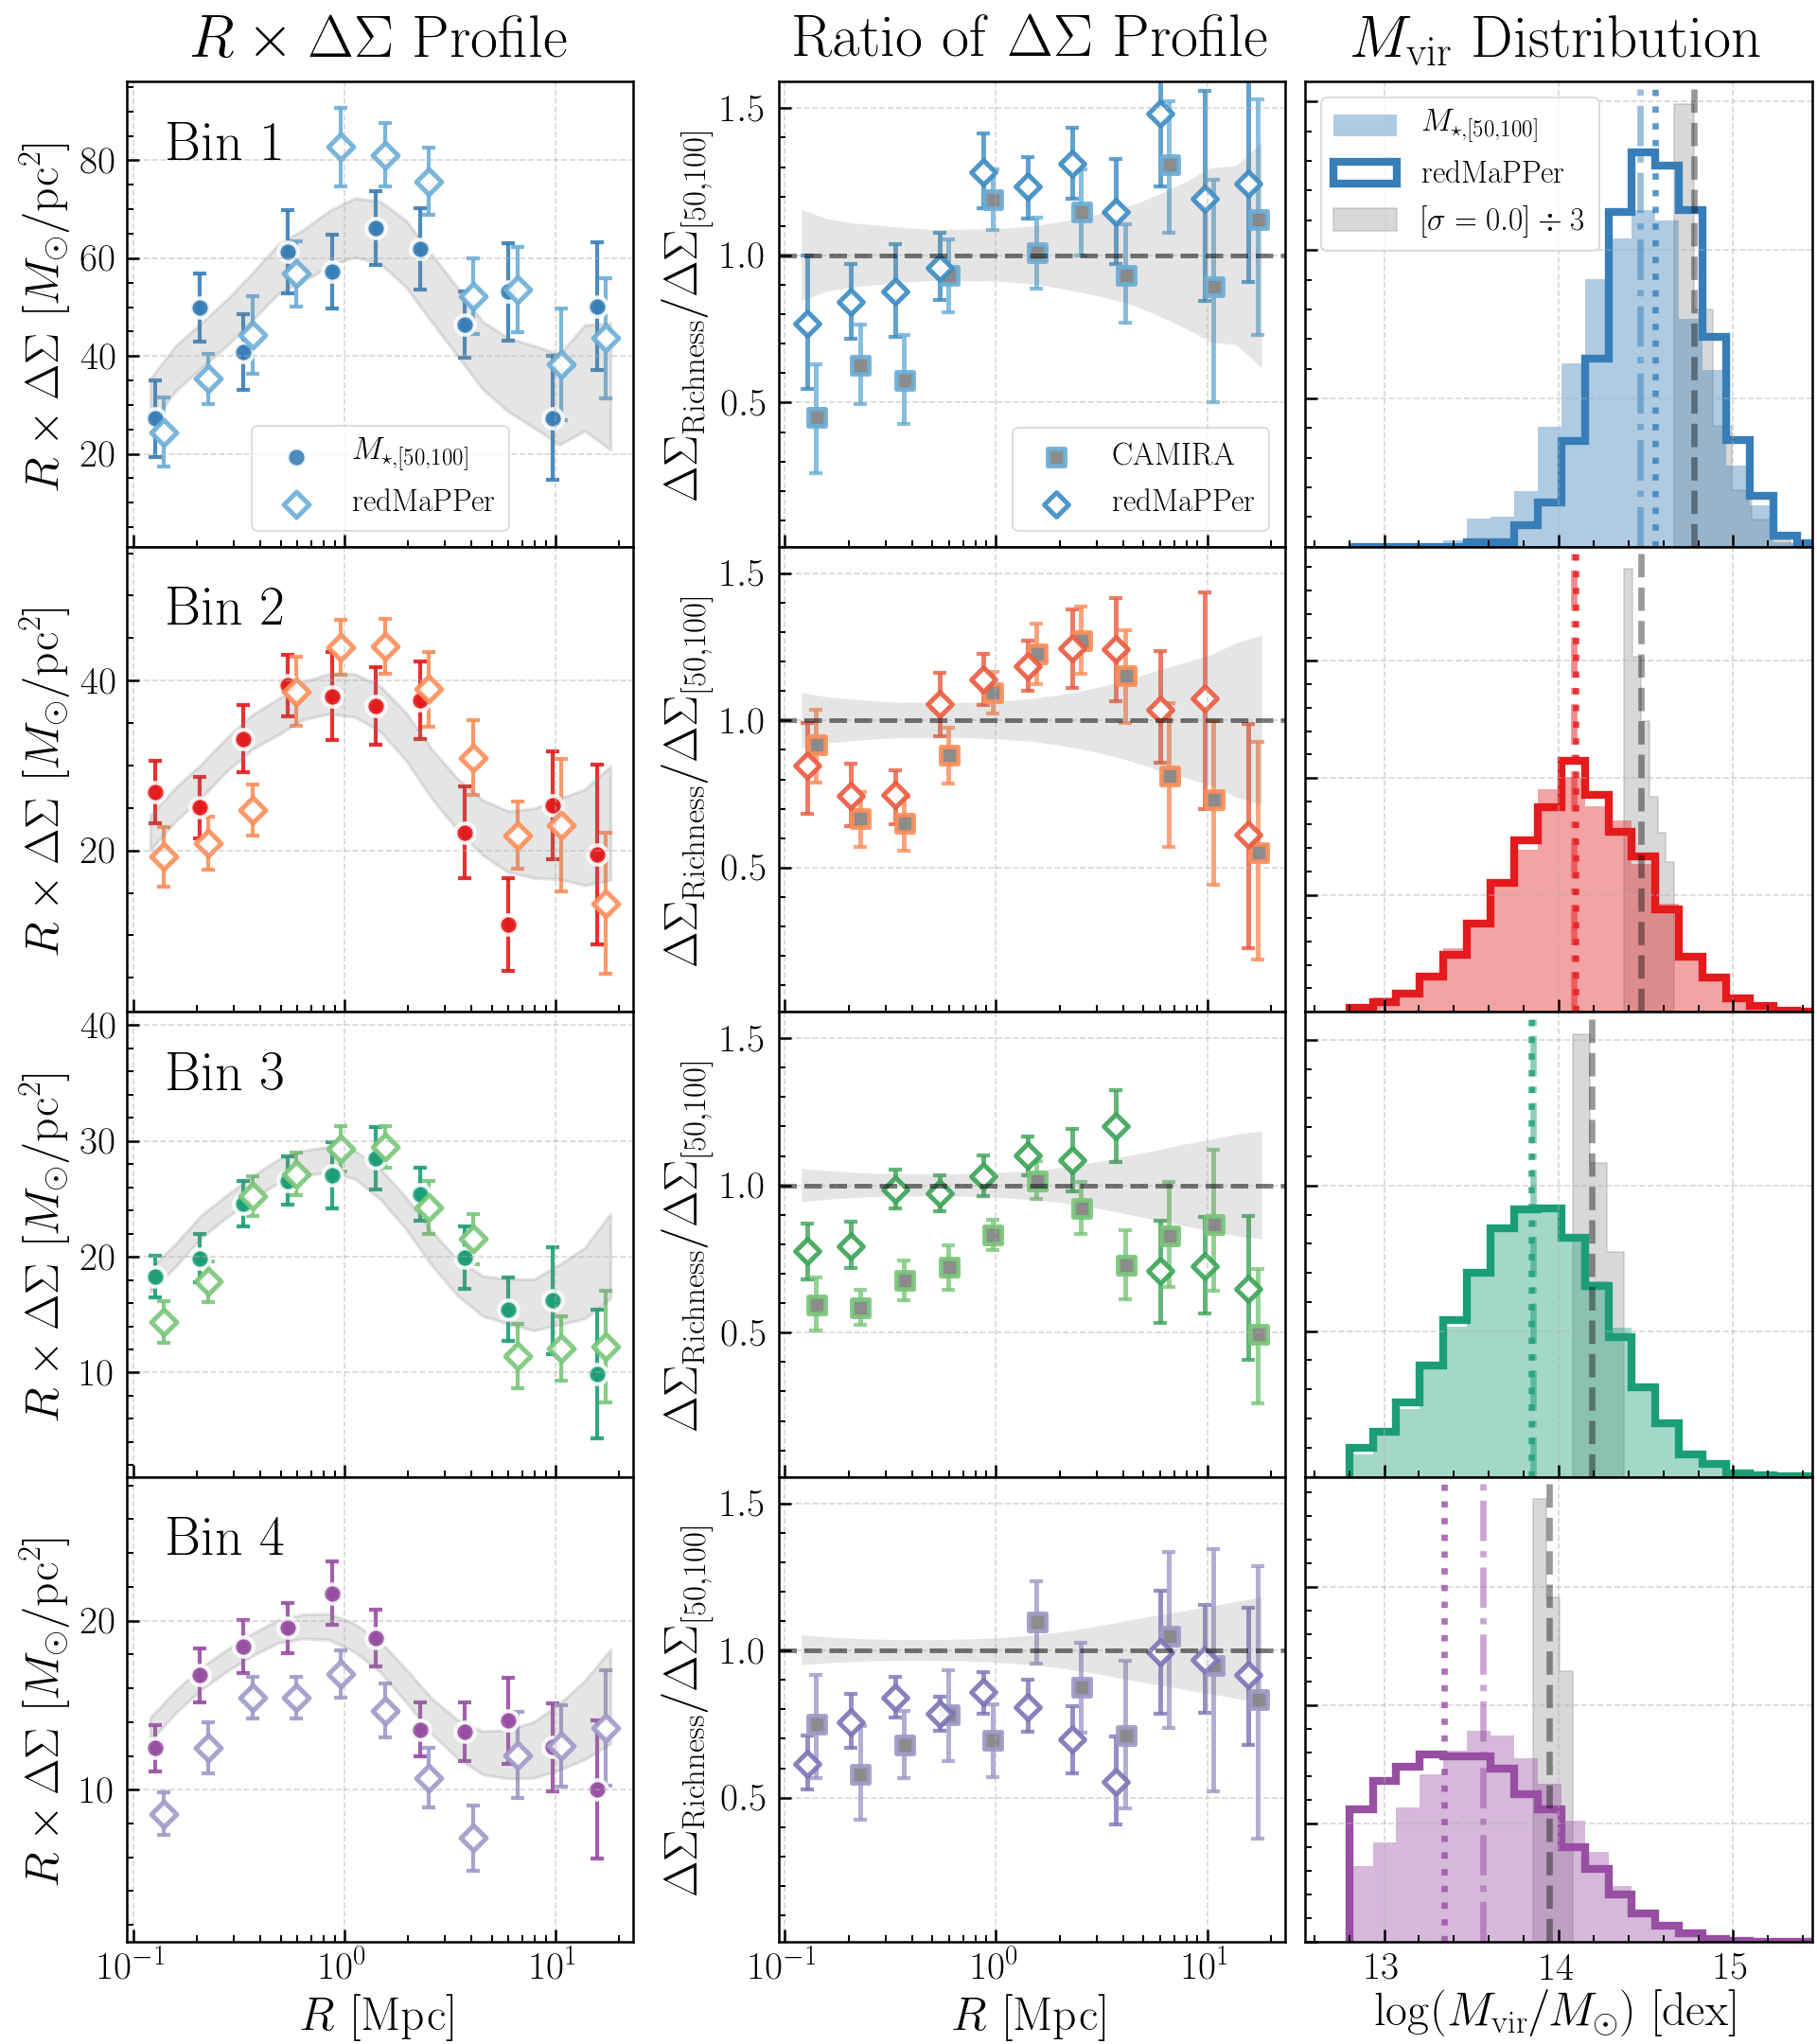
\includegraphics[width=\textwidth]{figure/topn_dsigma_mout6_redm_compare}
      \caption{
          \todo{Compare 50-100 kpc outer envelope mass and richness selected clusters}
          }
      \label{fig:mout_richness}
  \end{figure*}
%% ---------------------------------------------------------------------------------------------- %%

%% ---------------------------------------------------------------------------------------------- %%
%% Figure: Compare the DSigma profiles of richness selection clusters with their 
%%		   best-fit model.
%% ---------------------------------------------------------------------------------------------- %%
  \begin{figure*}
      \centering
      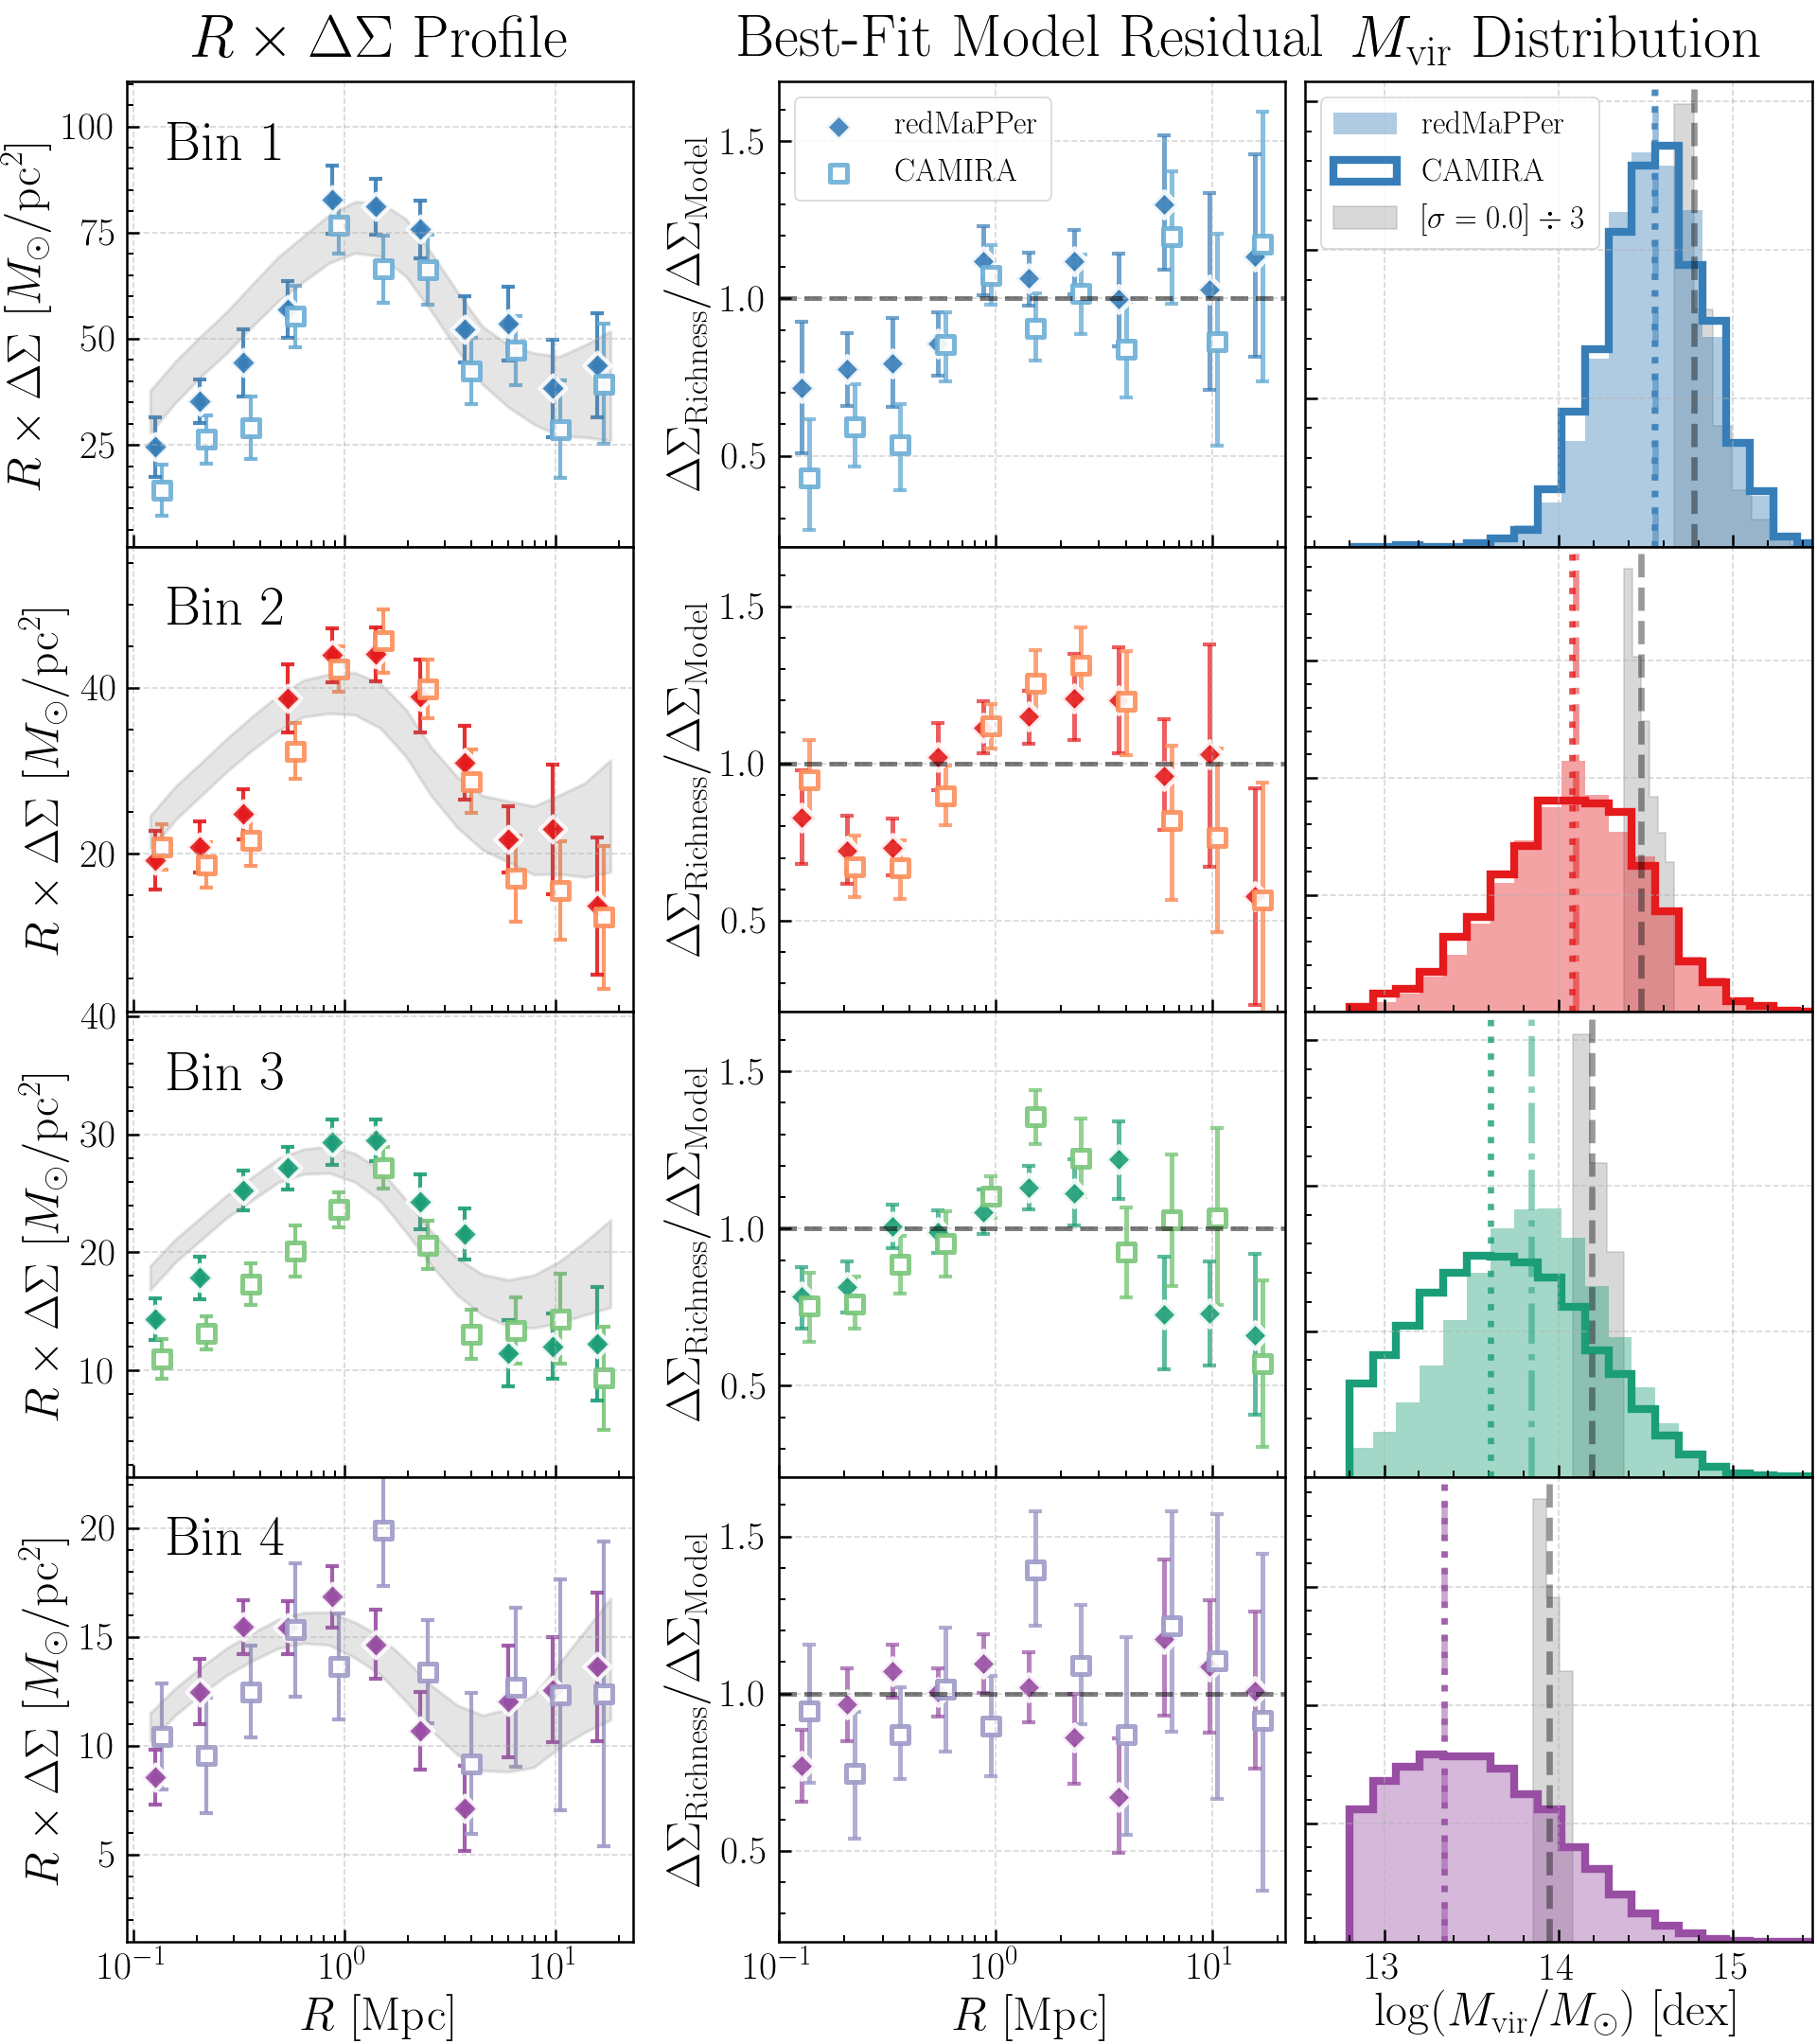
\includegraphics[width=\textwidth]{figure/topn_dsigma_redm_cam_residual}
      \caption{
          \todo{Compare the DSigma profiles of richness selection clusters with their 		   
          		best-fit model.}
          }
      \label{fig:richness_residual}
  \end{figure*}
%% ---------------------------------------------------------------------------------------------- %%

    
%% ---------------------------------------------------------------------------------------------- %%
%% Discussion 
%% ---------------------------------------------------------------------------------------------- %%
\section{Discussion}
    \label{sec:discussion}

\begin{itemize}
    \item How does this change how we think about optical cluster finding?
    \item Importance of measuring total luminosity. Crappiness of Cmodel. What are the current limitations.
    \item Chris paper: but selection by $M*$ could be more subject to assembly bias
    \item Baryonic effects can be discussed here
\end{itemize}


%% ---------------------------------------------------------------------------------------------- %%
%% Discussion about the outer envelope mass
%% ---------------------------------------------------------------------------------------------- %%
\subsection{Outer Galaxy Mass}

Discuss here why we think the outer mass may work the best. Is this because of the \textbf{slope}
of the $Mexsitu$ verus Mhalo plane being steeper than for insitu mass (see plot in Chris paper).
Can discuss how UM and TNG predictions are different in this regard.

Figure: show a figure of the ASAP model but using the outer mass. Is the boundary more clear? Is
this what ASAP was telling us all along?

%% ---------------------------------------------------------------------------------------------- %%
%% ---------------------------------------------------------------------------------------------- %%
\subsection{Comparison with \redm{} and other cluster finders}
    \label{sec:richness}

    \todo{Placeholder}
    
%% ---------------------------------------------------------------------------------------------- %%
%% ---------------------------------------------------------------------------------------------- %%
\subsection{Comparison with X--ray observation}
    \label{sec:xray}

\textbf{We are going to think about whether to add this here or not. Deceide later.}

    \todo{Placeholder}
    \song{Need to read more recent works on this}
\alexie{Let's discuss, what goes here?}

%% ---------------------------------------------------------------------------------------------- %%
%% Summary 
%% ---------------------------------------------------------------------------------------------- %%
\section{Summary and Conclusions}
    \label{sec:summary}
    
    % Main conclusion    
    \todo{Placeholder}    

    % Future direction   
    \todo{Briefly mention a few future directions. Also name as many as I can think of, 
          need to pick a few.}

%% ---------------------------------------------------------------------------------------------- %%
%% Acknowledgements 
%% ---------------------------------------------------------------------------------------------- %%
\section*{Acknowledgements}

  % Personal 
  \todo{The authors would like to thank XXX for useful discussions and suggestions.}

  % NSF funding
  This material is based upon work supported by the National Science Foundation under 
  Grant No. 1714610. 
  
  % KITP
  The authors acknowledge support from the Kavli Institute for Theoretical Physics.
  This research was also supported in part by National Science Foundation under Grant 
  No. NSF PHY11-25915 and Grant No. NSF PHY17-48958
  
  % AL's funding 
  We acknowledge use of the lux supercomputer at UC Santa Cruz, funded by NSF MRI grant AST
  1828315. AL is supported by the U.D Department of Energy, Office of Science, Office of High
  Energy Physics under Award Number DE-SC0019301. AL acknowledges support from the David and
  Lucille Packard foundation, and from the Alfred .P Sloan foundation.

  % HSC part
  The Hyper Suprime-Cam (HSC) collaboration includes the astronomical communities of 
  Japan and Taiwan, and Princeton University.  The HSC instrumentation and software were
  developed by National Astronomical Observatory of Japan (NAOJ), Kavli Institute
  for the Physics and Mathematics of the Universe (Kavli IPMU), University of Tokyo,
  High Energy Accelerator Research Organization (KEK), Academia Sinica Institute
  for Astronomy and Astrophysics in Taiwan (ASIAA), and Princeton University.  
  Funding was contributed by the FIRST program from Japanese Cabinet Office,  Ministry 
  of Education, Culture, Sports, Science and Technology (MEXT), Japan Society for 
  the Promotion of Science (JSPS), Japan Science and Technology Agency (JST), Toray 
  Science Foundation, NAOJ, Kavli IPMU, KEK, ASIAA, and Princeton University.
   
  % SDSS part
  Funding for SDSS-III has been provided by Alfred P. Sloan Foundation, the 
  Participating Institutions, National Science Foundation, and U.S. Department of
  Energy. The SDSS-III website is http://www.sdss3.org.  SDSS-III is managed by the
  Astrophysical Research Consortium for the Participating Institutions of the SDSS-III
  Collaboration, including University of Arizona, the Brazilian Participation Group,
  Brookhaven National Laboratory, University of Cambridge, University of Florida, the
  French Participation Group, the German Participation Group, Instituto de Astrofisica
  de Canarias, the Michigan State/Notre Dame/JINA Participation Group, Johns Hopkins
  University, Lawrence Berkeley National Laboratory, Max Planck Institute for
  Astrophysics, New Mexico State University, New York University, Ohio State University,
  Pennsylvania State University, University of Portsmouth, Princeton University, the
  Spanish Participation Group, University of Tokyo, University of Utah, Vanderbilt
  University, University of Virginia, University of Washington, and Yale University.
  
  % Pan-STARRS1 part
  The Pan-STARRS1 surveys (PS1) have been made possible through contributions of  
  Institute for Astronomy; University of Hawaii; the Pan-STARRS Project Office; 
  the Max-Planck Society and its participating institutes: the Max Planck Institute 
  for Astronomy, Heidelberg, and the Max Planck Institute for Extraterrestrial Physics, 
  Garching; Johns Hopkins University; Durham University; University of Edinburgh; 
  Queen's University Belfast; Harvard-Smithsonian Center for Astrophysics; Las 
  Cumbres Observatory Global Telescope Network Incorporated; National Central 
  University of Taiwan; Space Telescope Science Institute; National Aeronautics 
  and Space Administration under Grant No. NNX08AR22G issued through the Planetary 
  Science Division of the NASA Science Mission Directorate; National Science 
  Foundation under Grant No. AST-1238877; University of Maryland, and Eotvos 
  Lorand University. 
  
  % LSST software
  This research makes use of software developed for the Large Synoptic Survey 
  Telescope. We thank the LSST project for making their code available as free 
  software at http://dm.lsstcorp.org.
  
  % SMDPL simulation
  The CosmoSim database used in this research is a service by the Leibniz-Institute for 
  Astrophysics Potsdam (AIP).
  The MultiDark database was developed in cooperation with the Spanish MultiDark 
  Consolider Project CSD2009-00064.
  
  % Software
  This research made use of:
  \href{http://www.stsci.edu/institute/software_hardware/pyraf/stsci\_python}{\texttt{STSCI\_PYTHON}},
      a general astronomical data analysis infrastructure in Python. 
      \texttt{STSCI\_PYTHON} is a product of the Space Telescope Science Institute, 
      which is operated by Association of Universities for Research 
      in Astronomy (AURA) for NASA;
  \href{http://www.scipy.org/}{\texttt{SciPy}},
      an open source scientific tool for Python (\citealt{SciPy});
  \href{http://www.numpy.org/}{\texttt{NumPy}}, 
      a fundamental package for scientific computing with Python (\citealt{NumPy});
  \href{http://matplotlib.org/}{\texttt{Matplotlib}}, 
      a 2-D plotting library for Python (\citealt{Matplotlib});
  \href{http://www.astropy.org/}{\texttt{Astropy}}, a community-developed 
      core Python package for astronomy (\citealt{AstroPy}); 
  \href{http://scikit-learn.org/stable/index.html}{\texttt{scikit-learn}},
      a machine-learning library in Python (\citealt{scikit-learn}); 
  \href{https://ipython.org}{\texttt{IPython}}, 
      an interactive computing system for Python (\citealt{IPython});
  \href{https://github.com/kbarbary/sep}{\texttt{sep}} 
      Source Extraction and Photometry in Python (\citealt{PythonSEP});
  \href{https://jiffyclub.github.io/palettable/}{\texttt{palettable}},
      colour palettes for Python;
  \href{http://dan.iel.fm/emcee/current/}{\texttt{emcee}}, 
      Seriously Kick-Ass MCMC in Python;
  \href{http://bdiemer.bitbucket.org/}{\texttt{Colossus}}, 
      COsmology, haLO and large-Scale StrUcture toolS (\citealt{Colossus}).

%% ---------------------------------------------------------------------------------------------- %%
%% References  
%% ---------------------------------------------------------------------------------------------- %%
\bibliographystyle{mnras}
\bibliography{topn}

%% ---------------------------------------------------------------------------------------------- %%
%% Appendix Section
%% ---------------------------------------------------------------------------------------------- %%

\appendix

%% ---------------------------------------------------------------------------------------------- %%
%% More on the method of profile matching
%% ---------------------------------------------------------------------------------------------- %%
\section{Matching \dsigma{} profiles} 
	\label{app:fitting} 
    
    \todo{Placeholder}

%% ---------------------------------------------------------------------------------------------- %%
%% Figure: Demonstrate the scatter matching process.
%% ---------------------------------------------------------------------------------------------- %%
  \begin{figure*}
      \centering 
      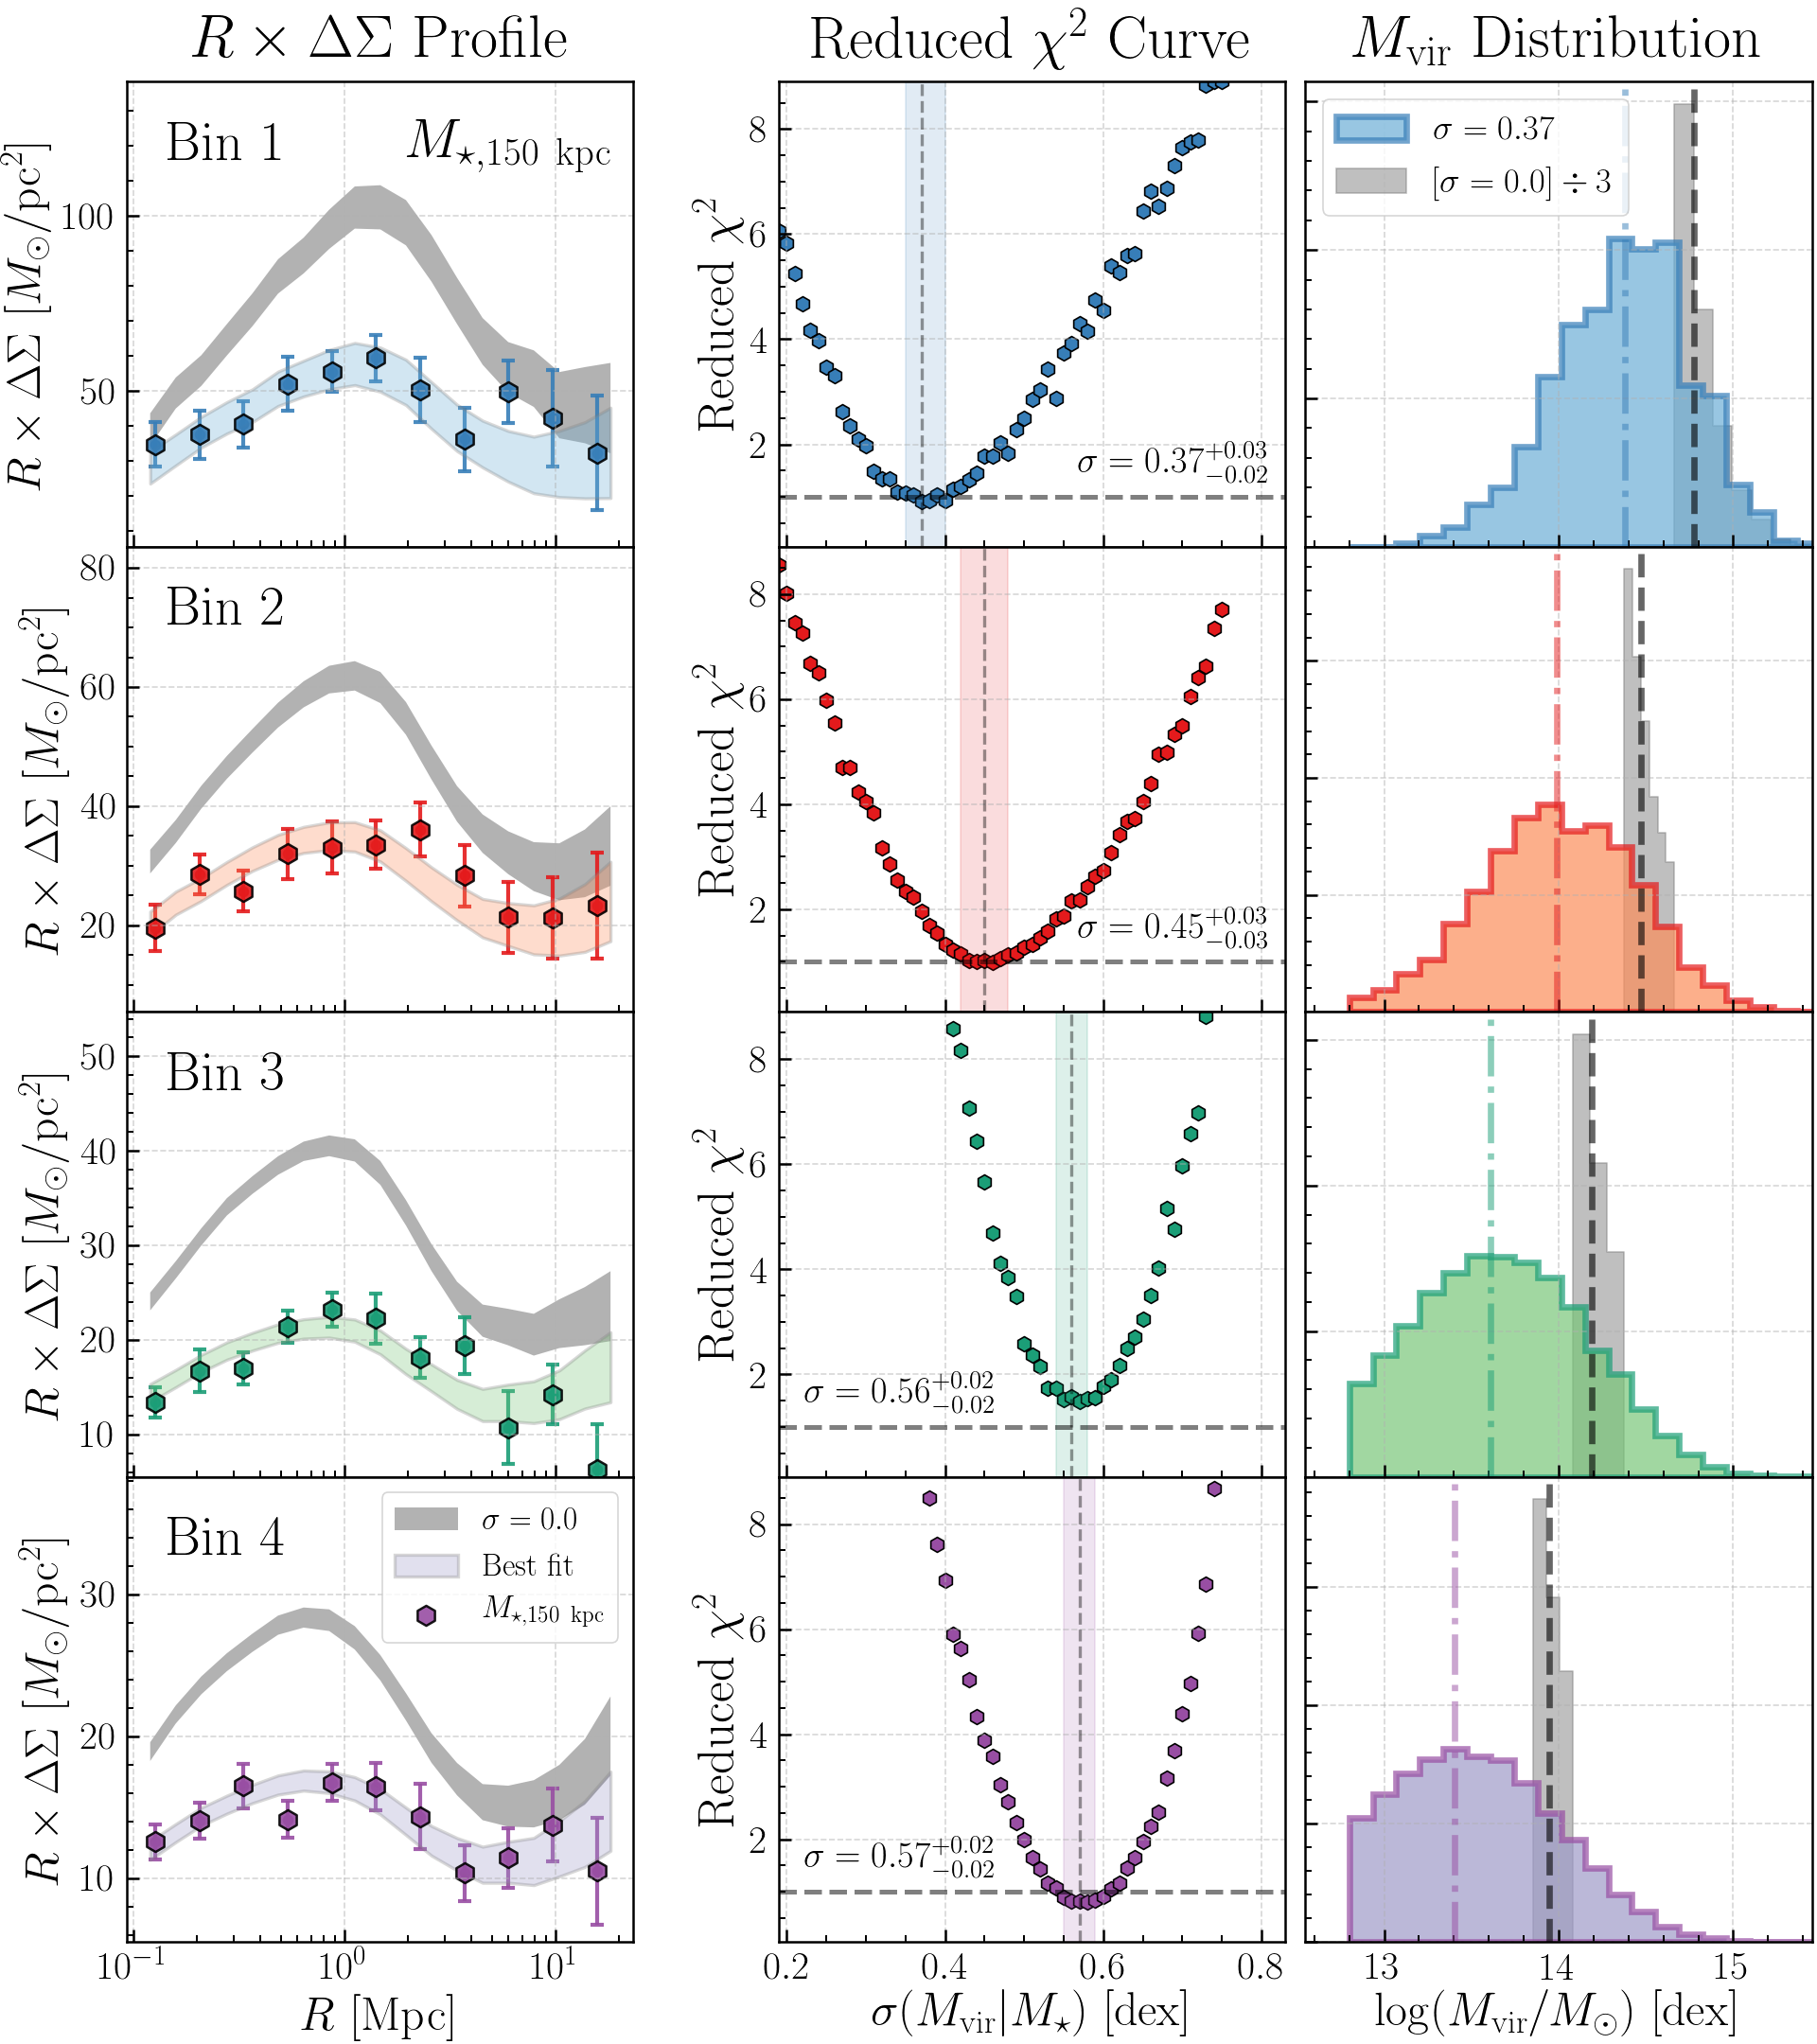
\includegraphics[width=\textwidth]{figure/topn_dsigma_m150_fit}
      \caption{
          \todo{Demonstrate the scatter matching process.}
          }
      \label{fig:fitting}
  \end{figure*}
%% ---------------------------------------------------------------------------------------------- %%
    

%% ---------------------------------------------------------------------------------------------- %%
%% Impact of P_cen on the DSigma profile of richness selected clusters
%% ---------------------------------------------------------------------------------------------- %%
\section{Impact of $P_{\rm cen}$ on the \dsigma{} profile of \redm{} clusters} 
	\label{app:pcen} 
    
    \todo{Placeholder}

%% ---------------------------------------------------------------------------------------------- %%
%% Figure: Impact of Pcen cuts on redMaPPer DSigma profiles.
%% ---------------------------------------------------------------------------------------------- %%
  \begin{figure*}
      \centering 
      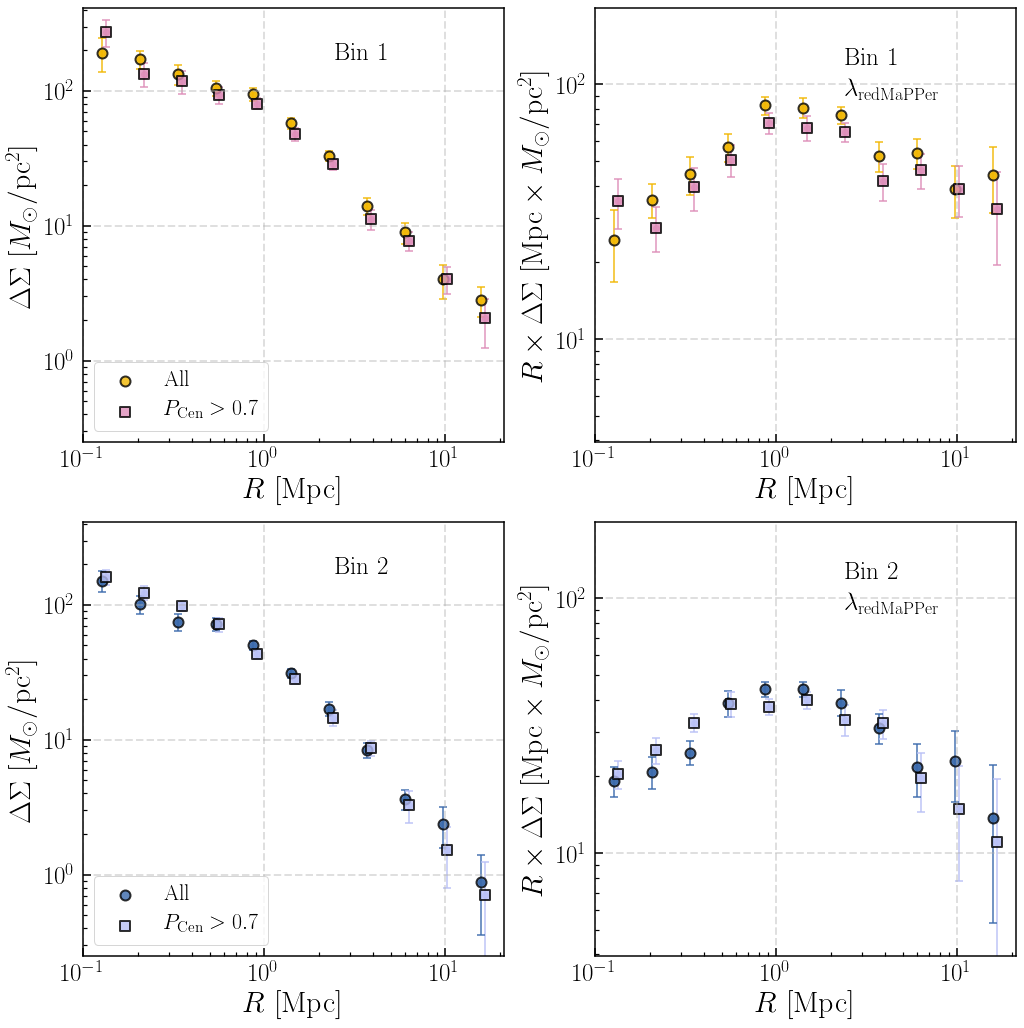
\includegraphics[width=12cm]{figure/redmapper_pcen_placeholder}
      \caption{
          \todo{PLACEHOLDER: Impact of $P_{\rm Cen\ 1}$ cuts on the \redm{} \dsigma{} profiles.
          (For appendix)}
          }
      \label{fig:pcen}
  \end{figure*}
%% ---------------------------------------------------------------------------------------------- %%

%% ---------------------------------------------------------------------------------------------- %%
%% Galaxy size as potential halo mass indicator
%% ---------------------------------------------------------------------------------------------- %%
\section{Galaxy Size as \mvir{} indicator} 
	\label{app:size} 
    
    \todo{Placeholder}


%% ---------------------------------------------------------------------------------------------- %%
\bsp
\label{lastpage}
\end{document}

%% ---------------------------------------------------------------------------------------------- %%
%% ------ End of the File ------
%% ---------------------------------------------------------------------------------------------- %%